\documentclass[10pt,a4paper]{article}

% PACKAGES
\usepackage{graphicx}
\usepackage{caption}
\usepackage{subcaption}
\usepackage[left=2.5cm,right=2.5cm,top=2.5cm,bottom=2.5cm,paperwidth=170mm,paperheight=240mm]{geometry} % Approximates 122mm x 193mm text area
\usepackage{fancyhdr}
\usepackage{parskip}
\usepackage{natbib}
\usepackage{imakeidx}
\usepackage{hyperref}
\usepackage{amsmath}
\usepackage[acronym]{glossaries}
\usepackage{lipsum} % DUMMY TEXT
\usepackage[english]{babel} % Assuming English
\usepackage{titlesec}
\usepackage{tabularx}
\usepackage{float}
\usepackage{setspace}
\usepackage{multirow}
\usepackage{array}
\usepackage{listings}
\usepackage{placeins}
\usepackage{longtable}
\usepackage{color}
\usepackage{xcolor}
\usepackage{booktabs}
\usepackage{makecell}

% CONFIGS
\pagestyle{plain}
\fancyfoot[C]{\thepage}
\hypersetup{
    pdfauthor = {Avishka Sathyanjana},
    pdftitle = {Multimodal Emotional State Recognition for Personalized Responses},
    colorlinks,
    linkcolor={black},
    citecolor={black}
}
\PassOptionsToPackage{unicode}{hyperref}

% MACROS
\newcommand{\unit}[1]{\ensuremath{\, \mathrm{#1}}}  % Makes writing units simpler
\renewcommand{\thefootnote}{\emph{\alph{footnote}}} % Italic letters for footnotes

% PATHS
\graphicspath{ {img/} }

% BIB SETUP
\bibliographystyle{plainnat} % Numerical citation style

% TITLE FORMAT
\title{\textbf{\fontsize{14}{16}\selectfont Multimodal Emotional State Recognition for Personalized Responses}}
\author{
    \fontsize{10}{12}\selectfont Avishka Sathyanjana \\
    \fontsize{9}{11}\selectfont University of Moratuwa, Sri Lanka \\
    \fontsize{9}{11}\selectfont avishka.sathyanjana@example.com
}

% HEADINGS FORMAT
\titleformat{\section}{\normalfont\large\bfseries}{\thesection}{1em}{}
\titleformat{\subsection}{\normalfont\normalsize\bfseries}{\thesubsection}{1em}{}
\titleformat{\subsubsection}{\normalfont\normalsize\bfseries}{\thesubsubsection}{1em}{}
\titleformat{\paragraph}{\normalfont\normalsize\bfseries}{\theparagraph}{1em}{}

% DOCUMENT BEGIN HERE
\begin{document}

% TITLE AND AUTHOR
\maketitle

% ABSTRACT
\begin{abstract}
    \fontsize{9}{11}\selectfont
  This study presents a personalized multimodal emotion recognition framework that adapts to individual emotional baselines using facial and vocal signals. Decision Level Fusion with Mean Squared Error assigns personalized weights based on user-reported emotions. Kernel Density Estimation establishes an initial arousal-valence baseline, refined via reinforcement learning with emoji-based feedback. Experiments with 10 participants across five emotions (Happy, Angry, Sad, Boredom, Calm) show the fused method improves accuracy by 33.92\% over facial and 6.52\% over vocal methods. Personalized responses enhanced empathy (75.3\%), emotional alignment (69.5\%), and satisfaction (37.6\%). Most participants (66.67\%) validated the refined baseline. Contributions include a personalized fusion method, baseline identification, and iterative refinement. Future work will expand emotional categories, incorporate physiological data, and enhance context-aware fusion. This framework advances personalized human-computer interaction.
\end{abstract}

% KEYWORDS
\textbf{Keywords:} Affective Computing, Emotional State Recognition, Multimodal Analysis, Personalized Responses, Machine Learning, Human-Computer Interaction, Reinforcement Learning, Arousal-Valence, 

% INTRODUCTION
\section{Introduction}
\par Affective computing is a multidisciplinary research area where computer science bridges the gap between cognitive science, psychology, and social science. It empowers intelligent systems to recognize, conclude, and interpret human emotions, facilitating better human-machine interaction by responding to
humans based on their emotional state \citep{picard2000affective}. Given the significant variability of emotional states across individuals, personalized emotion recognition models are essential, particularly for applications such as personal assistants where user satisfaction and engagement are paramount \citep{salama2020deep}.

\par However, despite advances in real-time emotion recognition, current systems often provide generic responses that fail to account for the dynamic and personalized nature of emotional experiences \citep{kim2024understanding}. This limitation arises because emotions are rooted in an individual's baseline emotional state, which represents their stable mood \citep{davidson1998affective}, yet most systems overlook this baseline, resulting in responses that may feel disconnected or inadequate. The root of this issue lies in the lack of longitudinal analysis and personalized baselines in existing systems, which compromises the accuracy of emotion identification by failing to account for individual emotional biases. 

\par To address this gap, this study develops a personalized multimodal emotion recognition framework that integrates facial and vocal signals to establish and refine individual emotional baselines. By employing Decision Level Fusion and reinforcement learning, the framework achieves greater accuracy in capturing emotions while adapting to individual differences. This approach not only enhances the precision of emotion recognition but also fosters responsive, empathetic, and adaptive interactions, with significant implications for domains such as mental health support, customer service, and adaptive learning. The research objectives are to develop this framework, evaluate its effectiveness in recognizing personalized emotional states, and assess its impact on the quality of responses generated by large language models.
\section{Research Aim, Questions and Objective}
\label{sec:research-aim-questions-objectives}

\subsection{Research Aim}
\label{subsec:research-aim}
\par To develop and evaluate a personalized emotion recognition framework that uses facial expressions and audio data to identify an individual's emotional baseline, with the goal of enhancing the emotional intelligence of LLM responses.

\subsection{Research Questions and Objectives}
\label{subsec:research-questions-objectives}

\textbf{Objective 1 - Develop a multi-modal emotional recognition framework with Personalized Arousal-Valence Identification}
\label{obj:1}    
\begin{itemize}
    \item \textbf{RQ 1.1:}\label{rq:1.1} What are suitable pre-implemented models that can be used to get a higher accuracy for emotion recognition?

    \item \textbf{RQ 1.2:}\label{rq:1.2} How the recognized emotion values from different modalities fused together in order to get more personalized arousal-valence value?
      
    \item \textbf{Approach:} Conduct a comprehensive literature review to identify suitable pre-trained ML models along with the suitable datasets for each modality. Participants will engage in emotion-eliciting tasks to gather real-time data, enabling fine-tuning of the fusion technique. User feedback will guide adjustments, refining the model to accurately capture personalized arousal-valence values, thereby enhancing the system's adaptability to individual emotional responses.
\end{itemize}

\textbf{Objective 2 - Identify Initial Baseline and Implement Dynamic Personalized Baseline Identification Using Reinforcement Learning Iterations}
\label{obj:2}
\begin{itemize}
    \item \textbf{RQ 2.1:}\label{rq:2.1} What techniques are most suitable for establishing an initial emotional baseline and how can this baseline be dynamically adjusted over time to reflect changes in the user's emotional responses and self-reported feedback?
    
    \item \textbf{Approach:} Begin by evaluating various techniques to determine the best fit for identifying an initial emotional baseline using data from emotional-eliciting tasks. Implement an iterative adjustment process where participant feedback and ongoing data inputs help refine the baseline over time. This approach enables the model to dynamically adapt to individual users.
\end{itemize}


\textbf{Objective 3 - Integrate the personalized emotional state information with user queries and measure the impact on the quality of responses generated by a LLM, compared to a control condition without emotional state input}
\label{obj:3}
\begin{itemize}
    \item \textbf{RQ 3.1:}\label{rq:3.1} How does integrating personalized emotional state information with user queries affect the relevance and user satisfaction of responses from LLMs?
    
    \item \textbf{Approach:} Participants will interact with a LLM by providing queries and receiving two responses: one from passing the raw query to the LLM (control condition), and another one combining the personalized emotional state information along with the user query (experimental condition).
\end{itemize}
\section{Research Methodology }

\subsection{Research Approach}
\par The planned approach for this research is a combined approach using \textbf{Action research and mixed methods}.
\newline
Action research is suitable for this research because we plan to use iterative cycles of action, observations, and the participatory nature of the research. Participants feedback and information will continuously refine the emotion baseline recognition system, ensuring the research addresses practical challenges and generates actionable knowledge.(figure \ref{fig:action})
\newline 
The mixed-methods approach integrates quantitative data with qualitative insights, providing a comprehensive evaluation of the framework's effectiveness. Quantitative data will be used to train and validate the machine learning model, while qualitative feedback will offer deeper insights into the participants' experiences and the system's practical applicability. 

\begin{figure*}[h]
\centering
\includegraphics[width=1\textwidth]{img/chapter_01/action-plan.jpg}
\captionof{figure}{Action Plan}
\label{fig:action}
\end{figure*}
\section{Scope}
\subsection{In Scope}
\begin{enumerate}
    \item Use existing pre-trained models for multimodal emotion recognition
        \begin{itemize}
            \item Our key contribution lies in effectively combining facial and audio emotion recognition modalities. By fusing data from facial and audio inputs, we can cross-validate and enhance overall emotion detection accuracy.
        \end{itemize}
    \item Develop personalized, adaptive emotional baselines model
        \begin{itemize}
            \item Many emotion recognition systems use universal, static baselines, leading to inaccuracies as individual behaviors change over time. Our innovative approach is to establish and continuously update personalized baselines for each user.
        \end{itemize}
    \item Develop an application that captures data to recognize the user's emotional state and facilitates interaction with large language models.
        \begin{itemize}
            \item This application will use prompt engineering to combine the user's emotional state with their query, enhancing the relevance and personalization of the responses from the LLM.
        \end{itemize}
\end{enumerate}

\subsection{Delimitations}
\begin{enumerate}
    \item Develop new facial and audio emotion modals from scratch
        \begin{itemize}
            \item Given the abundance of highly accurate, well-established models in each domain, reimplementing these is unnecessary. Our focus is on multimodal integration and personalization, not on improving individual modalities.
        \end{itemize}
    \item Modify core AI models (GPT architecture)
        \begin{itemize}
            \item Our scope is to enhance LLM responses by providing emotional context, not to alter the fundamental architecture of LLMs.
        \end{itemize}
    \item Making a dataset suited to the cultural context of Sri Lankans.
\end{enumerate}

% LITERATURE REVIEW
\section{Literature Review}
\section{Background and Related Work}
\label{sec:background}

\par Emotions are complex experiences of consciousness, bodily sensation, and behavior that reflects the personal significance of a thing, or an event. Plutchik introduced the Wheel of Emotions, a model that identifies eight fundamental emotions: joy, sadness, trust, disgust, fear, anger, anticipation, and surprise. According to this model, these basic emotions can combine in varying intensities to form more complex emotional states. Others are overlapping those fundamental emotions which can be seen in Figure~\ref{fig:wheel}. This research is the base for upcoming research in emotion categorization \citep{plutchik1980general}. Valence-Arousal-Dominance (VAD) model represents emotions along three dimensions: pleasantness (valence), activation (arousal), and control (dominance). It provides a simple and intuitive way to understand the different components of emotion Figure~\ref{fig:two-dim}. \citep{oberlander2018analysis}.

\begin{figure*}[h]
\centering
\begin{subfigure}[b]{0.45\textwidth}
    \includegraphics[height=2.56in,width=2.56in]{img/wheel-of-emotions.jpg}
    \caption{Wheel of emotions}
    \label{fig:wheel}
\end{subfigure}
\hfill
\begin{subfigure}[b]{0.45\textwidth}
    \includegraphics[height=2.4in,width=3.35in]{img/two-dim-modal.png}
    \caption{Russell's two-dimensional model of valence and arousal}
    \label{fig:two-dim}
\end{subfigure}
\caption{Emotion categorization}
\label{fig:combined}
\end{figure*}

\par These emotions are expressed using both verbal and nonverbal channels. As \cite{ekman1971constants} showed, facial expressions universally convey six basic emotions across cultures. Our voices carry emotional information through tone, pitch, and pace, with high-arousal emotions often involving higher pitch and faster pace (Barrett, 2004). Body language, such as posture and gestures, also communicates emotional states \citep{ekman1971constants}. Verbally, we directly express our feelings using linguistic patterns and exact words reflecting higher emotional granularity \citep{smidt2015brief}. In today's digital age, we frequently express emotions in text, a focus of sentiment analysis in natural language processing \citep{lim2016cultural}. Physiological changes like increased heart rate also signal emotions, particularly their arousal levels \citep{barrett2004journal}. 

\par However, the expression of the emotions varies significantly from person to person and across different cultures. Emotional granularity, which is a factor in this variability, is the ability to make fine-grained distinctions between similar emotions \citep{smidt2015brief}. The cultural differences profoundly influence emotional arousal and expression. For instance, research by \citep{lim2016cultural} highlights that Western cultures tend to value and promote high-arousal emotions such as excitement and anger, whereas Eastern cultures prioritize low-arousal emotions like calmness and contentment. Because of that, it’s important to establish a baseline behavior of individuals in advance to identify their emotional state in a more precise manner.

\par Baseline behavior refers to an individual's typical or normal pattern of behavior, thoughts, and emotions when they are not experiencing any specific external stimuli or circumstances that would significantly influence their state. It represents the default or resting state from which deviations or changes can be measured. Emotional baseline, also known as emotional homeostasis or emotional equilibrium, is the relatively stable state of emotional experience that an individual tends to return to after experiencing temporary emotional fluctuations. It is the individual's characteristic or typical level of emotional arousal and emotional experience when not influenced by external events or stimuli. \citep{davidson1998affective} 












\section{Facial Emotion Recognition}
\label{sec:fer}
\par Facial expressions occur by contracting and releasing of the muscles under the skin. Most existing applications use the movements of facial muscles considering action units and this uses supervised learning approach which is known as Facial Action Coding System (FACS) \citep{kantharia2015facial}. By using the CNN, the emotion recognition can be done in real time. This Technology is known as Facial Expression Recognition using CNN (FERC). FERC has two parts, first it removes background and noises from the source and second part entirely focuses on extracting facial features. FERC model uses Expressional Vector to identify the basic emotions, and this was able to achieve 96\% accuracy \citep{mehendale2020facial}

\par in this research our interest is mostly on the continuous emotion prediction models rather than distinct emotion classification models. Study done by \cite{savchenko2024hsemotion} proposes EmotiEffNet family of models (a series of pre-trained convolutional networks) for valence-arousal prediction. These networks extract frame-level features which are fed into a Multi Layer Perceptron (MLP) and a LightAutoML classifier ensemble, with a post-processing step using smoothing to stabilize results across sequential frames. The Aff-Wild2 \citep{kollias2018aff} dataset is used in this study. Model achieved a valence CCC of 0.5603 and an arousal CCC of 0.5597 on the Aff-Wild2 dataset. This model is efficient in terms of computational requirements, reaching 45 FPS on a GPU and 12 FPS on a CPU, with a model size of 15MB, making it adaptable for mobile deployment.

\par The MaxViT model \citep{wagner2024cage} utilizes a hybrid approach, combining continuous valence-arousal labels with discrete emotion categories to train a transformer-based architecture. This circumplex model-guided inference provides a more nuanced approach by learning from both types of labels, thus enhancing expression recognition accuracy. The model is trained with AffectNet \citep{mollahosseini2017affectnet} and EMOTIC \citep{kosti2019context} datasets. CAGE achieved a CCC of 0.716 for valence and 0.642 for arousal on AffectNet, with a root mean square error (RMSE) reduction of 7\% for valence and 6.4\% for arousal. This model has a larger footprint, with a size of 86MB, and processes at 30 FPS on a GPU and 8 FPS on a CPU, making it suitable for high-end applications where computational resources are available.

\par Study done by \cite{savchenko2023emotieffnets} introduce EmotiEffNet model which leverages the EfficientNet-B0 architecture for frame-level feature extraction, followed by an MLP and LightAutoML classifier ensemble for downstream emotion analysis tasks. This approach is applied to predict VA, FER, and AU tasks within the video frames. Aff-Wild2 is again the primary dataset and the model achieves a valence CCC of 0.494 and an arousal CCC of 0.607. For FER, the F1 score reaches 0.433, while the AU detection F1 score is 0.486. This balance between accuracy and computational efficiency results in an inference speed of 40 FPS on GPU and 15 FPS on CPU, with a model size of 23MB, providing a suitable option for applications needing moderate computational efficiency.

\begin{table}[h!]
\centering
\caption{Comparison of Suitable Datasets}
\begin{tabularx}{\textwidth}{|>{\raggedright\arraybackslash}X|>{\raggedright\arraybackslash}X|>{\raggedright\arraybackslash}X|>{\raggedright\arraybackslash}X|>{\raggedright\arraybackslash}X|}
\hline
\textbf{Aspect} & \textbf{AffWild2} & \textbf{AffectNet} & \textbf{EMOTIC} & \textbf{Hume Facial Dataset} \\
\hline
\textbf{Total Frames/Images} 
    & 2.8M frames (545 videos) 
    & 320,739 (train) + 41,406 (val) 
    & 23,266 (train) + 7,203 (test) 
    & 452,783 mimic images + 534,459 judgments \\ 
\hline
\textbf{Annotations} 
    & VA (-1 to +1), 8 expressions, 12 AUs 
    & 8 expressions, VA (-1 to +1) 
    & 26 expressions, VA, arousal, dominance 
    & 28+ continuous emotional dimensions \\ 
\hline
\textbf{Resolution} 
    & Varying (in-the-wild) 
    & High-resolution 
    & Context-rich, full-body 
    & 160x160 pixels (standardized) \\ 
\hline
\textbf{Annotators} 
    & Expert-labeled 
    & 12 professionals 
    & Multi-annotator settings 
    & 5,833 participants (6 countries) \\ 
\hline
\textbf{Key Features} 
    & Video-based dynamic expressions 
    & Large-scale static images 
    & Contextual full-body analysis 
    & Cross-cultural mimicry, controls for demographic bias \\ 
\hline
\end{tabularx}
\label{tab:dataset_comparison}
\end{table}

\par A comparison of suitable datasets for our study is shown in Table~\ref{tab:dataset_comparison}.
These datasets vary in terms of labeled expressions, complexity, and real-world applicability. While AffWild2 and AffectNet focus on detailed face annotations, EMOTIC extends beyond facial analysis to include body language in contextual settings.

\par Hume.ai has developed sophisticated facial expression analysis technology centered on "semantic space theory,"\citep{cowen2021semantic} which enables a high-dimensional, data-driven understanding of human emotional expressions. This approach transcends traditional models by capturing hundreds of dimensions of human expression, allowing for the identification of subtle emotional nuances. Their Facial Expression Model identifies over 28 distinct facial expressions by analyzing millions of natural facial expressions collected from a diverse global population across six countries (USA, China, India, Venezuela, Ethiopia, and South Africa), comprising over 452,783 participant-generated mimic images and 534,459 emotion judgments from 5,833 participants. This extensive cross-cultural dataset deliberately controls for demographic variables to isolate genuine emotional signals, addressing limitations of culturally homogeneous samples in previous research.\citep{brooks2024deep}

\par The technology relies on a DNN model built on a FaceNet Inception ResNet v1 architecture pretrained on the VGGFace2 dataset that specifically analyzes facial features. Their FACS 2.0 Model provides an enhanced automated version of the Facial Action Coding System that measures 26 facial action units and 29 other facial features, offering detailed breakdown of facial movements that contribute to emotional expressions. The company employs principal preserved components analysis (PPCA) and generalized PPCA (G-PPCA) to extract 28 shared or culture-specific emotional dimensions from facial data. Unlike traditional models constrained to basic emotion categories, Hume.ai's system evaluates performance via correlation with human ratings of facial expressions rather than conventional metrics, ensuring alignment with real-world emotional interpretations while minimizing demographic biases\citep{brooks2024deep}.

Hume.ai's expression measurement technology is particularly valuable for practical applications through its WebSocket-based streaming capabilities, which facilitate real-time data processing without burdening local machines. This API-based approach enables continuous data flow between applications and Hume's models, providing immediate feedback on facial expressions through persistent two-way communication optimized for high throughput and low latency \citep{hume_api_2025}. The system can process various media formats with reasonable size limits (images up to 3,000 x 3,000 pixels, video up to 5 seconds) and offers both REST endpoints for batch processing and WebSocket endpoints for real-time predictions from sources like webcam streams. This infrastructure makes the sophisticated facial analysis technology highly accessible for applications requiring instant processing such as live customer service tools with the computational complexity handled on Hume.ai's servers rather than client devices \citep{hume_expression_2025a}.

% \begin{table}[h!]
% \centering
% \caption{Comparison of Emotion Recognition Models}
% \begin{tabularx}{\textwidth}{|X|X|X|X|}
% \hline
% \textbf{Aspect} & \textbf{MT-EmotiDDA MFN} & \textbf{MaxViT} & \textbf{EmotiEffNet} \\
% \hline
% Dataset & Aff-Wild2 & AffectNet, EMOTIC & Aff-Wild2 \\
% \hline
% Model Architecture & MobileNetV3 (lightweight MTL) & MaxViT (transformer-based hybrid) & EfficientNet-B0 with MLP ensemble \\
% \hline
% Valence CCC & 0.5603 & 0.716 & 0.494 \\
% \hline
% Arousal CCC & 0.5597 & 0.642 & 0.607 \\
% \hline
% Combined P\_VA Score & 0.5600 & Not specified & 0.550 \\
% \hline
% FER F1-score & 0.433 & Not specified & 0.433 \\
% \hline
% AU F1-score & 0.486 & Not specified & 0.486 \\
% \hline
% Post-processing & Gaussian/Box filters & Not specified & Box filtering for smoothing \\
% \hline
% Suitability & Real-time, mobile deployment & High-end applications & Moderate real-time applications \\
% \hline
% \end{tabularx}
% \label{tab:model_comparison}
% \end{table}

\begin{table}[h!]
\centering
\caption{Comparison of Emotion Recognition Models}
\begin{tabularx}{\textwidth}{|>{\raggedright\arraybackslash}X|>{\raggedright\arraybackslash}X|>{\raggedright\arraybackslash}X|>{\raggedright\arraybackslash}X|>{\raggedright\arraybackslash}X|}
\hline
\textbf{Aspect} & \textbf{MT-EmotiDDA MFN} & \textbf{MaxViT} & \textbf{EmotiEffNet} & \textbf{Hume Facial Expression} \\
\hline
Dataset 
    & Aff-Wild2 
    & AffectNet, EMOTIC 
    & Aff-Wild2 
    & Hume Facial Dataset \\
\hline
Model Architecture 
    & MobileNetV3 (lightweight MTL) 
    & MaxViT (transformer-based hybrid) 
    & EfficientNet-B0 with MLP ensemble 
    & FaceNet Inception ResNet v1 \\
\hline
Post-processing 
    & Gaussian/Box filters 
    & Not specified 
    & Box filtering for smoothing 
    & MTCNN face detection, 160x160 pixel standardization  \\
\hline
Suitability 
    & Real-time, mobile deployment 
    & High-end applications 
    & Moderate real-time applications 
    & Cross-cultural, Real time\\
\hline
\end{tabularx}
\label{tab:model_comparison}
\end{table}

The table~\ref{tab:model_comparison} provides a summarized, side-by-side comparison of each model's architecture, performance metrics, inference efficiency, and suitability for specific use cases, highlighting key findings.

\section{Speech Emotion Recognition} 
\label{sec:ser}
\par Our study focusing on identify the arousal valence values of speech emotions. Although there are many categorical datasets in SER, Only few has data with arousal, valence labeled and also in English language. Table~\ref{tab:ser_datasets} shows a detailed comparison on available SER datasets.

% \begin{table}[h!]
% \centering
% \begin{tabularx}{\textwidth}{|X|X|X|X|}
% \hline
% \textbf{Dataset} & \textbf{Year} & \textbf{Content} & \textbf{Emotions} \\
% \hline
% RAVDESS & 2018 & 7,356 recordings by 24 actors & 7 emotions: calm, happy, sad, angry, fearful, surprise, disgust \\
% \hline
% MuSe-CAR & 2021 & 40 hours, 6,000+ recordings of 25,000+ sentences by 70+ speakers & Continuous dimensions: valence, arousal, trustworthiness \\
% \hline
% Morgan Emotional Speech Set & 2019 & 999 spontaneous voice messages from 100 speakers & Valence , arousal, 4 emotions: happiness, anger, sadness, calm \\
% \hline
% OMG Emotion & 2018 & 420 videos, avg. length 1 min & 7 emotions: anger, disgust, fear, happy, sad, surprise, neutral; plus valence, arousal \\
% \hline
% IEMOCAP & 2007 & 12 hours, 5 sessions, 10 actors & Neutral, happiness, sadness, anger, surprise, fear, disgust, frustration, excited; Balanced: happiness, anger, sadness, frustration, neutral; 3 dimensions: valence, arousal, dominance \\
% \hline
% \end{tabularx}
% \caption{Comparison of Speech Emotion Recognition Datasets}
% \end{table}
 
\begin{table}[h!]
\centering
\begin{tabularx}{\textwidth}{|X|X|X|X|}
\hline
\textbf{Dataset} & \textbf{Year} & \textbf{Content} & \textbf{Emotions} \\
\hline
RAVDESS 
    & 2018 
    & 7,356 recordings by 24 actors 
    & 7 emotions: calm, happy, sad, angry, fearful, surprise, disgust \\
\hline
MuSe-CAR 
    & 2021 
    & 40 hours, 6,000+ recordings of 25,000+ sentences by 70+ speakers 
    & Continuous dimensions: valence, arousal, trustworthiness \\
\hline
Morgan Emotional Speech Set 
    & 2019 
    & 999 spontaneous voice messages from 100 speakers 
    & Valence, arousal, 4 emotions: happiness, anger, sadness, calm \\
\hline
OMG Emotion 
    & 2018 
    & 420 videos, avg. length 1 min 
    & 7 emotions categories; valence, arousal \\
\hline
IEMOCAP 
    & 2007 
    & 12 hours, 5 sessions, 10 actors 
    & 15 emotion categories; valence, arousal and dominance \\
\hline
HUME-VB 
    & 2023 
    & 282,906 vocalizations from 4,080 participants across 5 countries 
    & 48 emotion categories and 24 emotional dimensions \\
\hline
HUME-Prosody 
    & 2023 
    & 5,000+ "seed" samples and 282,906 trials of crowd-sourced mimicry responses across English, Mandarin, Spanish, Hindi 
    & 48 emotion categories with continuous  values \\
\hline
\end{tabularx}
\caption{Comparison of Speech Emotion Recognition Datasets}
\label{tab:ser_datasets}
\end{table}

\par The study \cite{zhang2017speech} utilizes the IEMOCAP dataset with CNNs for emotion recognition, extracting MFCCs, pitch, and prosodic features. The model achieved better performance on high-arousal emotions like anger and happiness but had challenges with neutral, low-arousal states. CNNs effectively captured emotional features relevant to both arousal and valence dimensions, highlighting the importance of carefully selected acoustic features in SER.

\par Another study done by \cite{martinez2020msp} Leveraging the MSP-Podcast corpus with time-continuous annotations, this study applied RNNs, particularly LSTMs, to capture sequential dependencies in speech emotions. By modeling continuous changes in emotions, the model achieved high correlation scores in arousal and valence prediction, making it well-suited for applications where emotions evolve over time.

\par Using the RAVDESS dataset, the study \cite{jalal2019spatio} explored LSTMs to enhance emotion detection, especially for low-arousal states. Focusing on features like pitch, energy, and spectral elements, the LSTM-based model demonstrated effectiveness in classifying nuanced emotions, achieving significant accuracy gains on emotions with subtle arousal shifts. The study supports the use of LSTMs in capturing temporal patterns, particularly for more subtle, low-arousal emotions.

\par This recent study \cite{wagner2023dawn} applied transformer architectures like wav2vec 2.0 and HuBERT, pre-trained on large audio datasets, for SER across MSP-Podcast, IEMOCAP, and MOSI. Transformers achieved state-of-the-art performance in valence recognition, with results revealing robust performance across diverse conditions and fairness in gender representation. The study showed that fine-tuning transformers with continuous annotations allows them to implicitly capture linguistic cues, which significantly improves valence prediction. 

\par Hume.ai's Vocal Burst dataset (HUME-VB) represents a groundbreaking resource for emotion recognition research, comprising 282,906 vocalizations from 4,080 participants across five culturally diverse countries (USA, China, India, Venezuela, South Africa) spanning multiple languages (English, Mandarin, Spanish, Hindi). This extensive dataset captures emotional expressions in real-world conditions with varied recording environments, making it the largest of its kind. The dataset has been leveraged in two significant ways: first, done by \cite{brooks2023vocalburst_deep} to train DNNs that predict 48 emotion categories from vocal bursts, revealing that nonverbal vocalizations express 24 distinct emotional dimensions with 79\% cross-cultural consistency, supporting Semantic Space Theory which conceptualizes emotions as continuous multi-dimensional states rather than discrete categories. Second done by \cite{tzirakis2023large_vocalburst}, used the dataset to develop transformer-based models, particularly Whisper architectures for detecting and classifying 67 vocalization types in audio streams, with the best-performing models achieving F1-scores of 96.2\% even in challenging noisy environments. These studies demonstrate the HUME-VB dataset's value in advancing understanding of cross-cultural emotional communication while providing practical applications for affective computing technology.

\par Hume.ai's Speech Prosody dataset (Hume-Prosody Corpus, HP-C) represents another significant contribution to emotional expression research, containing over 5,000 "seed" samples of emotional vocalizations and 282,906 trials of crowd-sourced mimicry responses collected across multiple languages (English, Mandarin, Spanish, Hindi) and cultures (USA, China, India, Venezuela, South Africa). This dataset was prominently featured in the 2023 Computational Paralinguistics Challenge (ComParE), where researchers tackled the "Emotion Share" task of predicting continuous emotion proportions across 48 emotion categories in speech segments \cite{schuller2023acm}. The challenge evaluated models using Spearman's rank correlation metrics, with baseline approaches including both modern transformer-based systems (Wav2Vec2) and traditional acoustic feature engineering (OpenSMILE). Research findings revealed that models struggled particularly with low-prevalence emotions, highlighting the need for balanced datasets, while also demonstrating significant cross-cultural variability in emotion expression. This work established important benchmarks for emotion share prediction while suggesting that future advances could come from combining acoustic and linguistic features, extending the dataset's utility for developing robust speech-based affective computing systems.

% Comparison of above studies is shown in table~\ref{tab:eye_summary}

\begin{table}[h!]
\centering
\begin{tabularx}{\textwidth}{|X|X|X|X|X|}
\hline
\textbf{Study} & \textbf{Dataset} & \textbf{Methodology} & \textbf{Key Results} & \textbf{Performance} \\
\hline
CNN on IEMOCAP & IEMOCAP & CNN, MFCC, pitch, prosodic & High accuracy on high-arousal & ~82\% for anger/happiness, ~65\% for neutral \\
\hline
RNN on MSP-Podcast & MSP-Podcast & RNN, LSTM, time-continuous annotation & Continuous tracking of emotions & Correlation: 0.403 (arousal), 0.196 (valence) \\
\hline
LSTM on RAVDESS & RAVDESS & LSTM, pitch, energy, spectral features & Low-arousal detection improved & 75\% accuracy for primary emotions, 68\% for low-arousal \\
\hline
Transformer-based Models on MSP-Podcast & MSP-Podcast, IEMOCAP, MOSI & Transformer (wav2vec 2.0, HuBERT) & Robust valence recognition, state-of-the-art on valence & CCC of 0.638 on MSP-Podcast for valence \\
\hline
\end{tabularx}
\caption{Comparison of Speech Emotion Recognition Studies}
\end{table}

\par In summary, emotion recognition research has evolved from foundational psychological theories like Plutchik’s wheel and the VAD model to sophisticated multimodal systems that analyze facial, vocal, and textual cues. Modern FER models such as EmotiEffNet and MaxViT demonstrate strong performance in valence-arousal prediction, balancing accuracy with computational efficiency. Hume.ai’s approach offers a culturally diverse and highly detailed understanding of emotional expression. Similarly, SER leverages CNNs, LSTMs, and transformers to model emotional variations in audio, with recent advances achieving state-of-the-art results using large, diverse datasets. Together, these developments underscore the importance of multimodal, culturally-aware, and continuously annotated datasets for advancing emotion recognition technologies.
\section{Multi-modal Fusion}
\par Multimodal analysis leverages input data from various channels like video, audio, and text to enhance the performance and accuracy of emotion recognition systems. The fusion of this multi-modal data is crucial, with techniques including feature-level fusion (combining features into one vector), decision-level fusion (independently classifying features and fusing outcomes), hybrid fusion (combining feature and decision-level approaches), model-level fusion (using correlations between models), rule-based fusion (assigning normalized weights), classification-based fusion (employing algorithms like SVMs and neural networks), and estimation-based fusion (useful for real-time audio and visual data, with filters like Kalman and particle filters). These fusion methods aim to effectively combine the data gathered from multiple modalities, enabling better emotional classification and recognition \citep{poria2017review}.


In summary, emotion recognition research has evolved from foundational psychological theories like Plutchik’s wheel and the VAD model to sophisticated multimodal systems that analyze facial, vocal, and textual cues. FER models such as EmotiEffNet and MaxViT demonstrate strong performance in valence-arousal prediction, balancing accuracy with computational efficiency. Hume.ai’s approach offers a culturally diverse and highly detailed understanding of emotional expression. Similarly, SER leverages CNNs, LSTMs, and transformers to model emotional variations in audio, with recent advances achieving state-of-the-art results using large, diverse datasets. Together, these developments underscore the importance of multimodal, culturally-aware, and continuously annotated datasets for advancing emotion recognition technologies.
\section{Reinforcement Learning Approaches for Personalized Applications}

Reinforcement Learning (RL) is a powerful method for building personalized systems. It helps systems to learn and improve based on user interactions over time. Many RL techniques have been used in different fields like entertainment, healthcare, education, and e-commerce. This section explains some popular RL approaches that are used for personalization.

\paragraph*{Contextual Bandits} This method is used by Netflix to show different artwork (thumbnails) for movies and series to different users. It learns from the user's past behaviour and decides which artwork will attract the user more. It balances between trying new options (exploration) and using known successful options (exploitation) \cite{netflix2018artwork}.

\paragraph*{Proximal Policy Optimization (PPO)} In healthcare, PPO has been used to suggest personalized cancer treatments. It works by ranking different drugs based on the data from each patient. This helps doctors to choose better treatments that match each patient's unique condition \cite{liu2022deep}.

\paragraph*{Deep Q-Learning (DQN)} DQN has been applied to recommend projects to users based on their interests. It improves the accuracy of recommendations and helps users to trust the system more \cite{wang2019personalized}.

\paragraph*{Q-Learning} This is a simple and popular RL method. It can be used for many general recommendation tasks and is good at adapting to changes in user preferences \cite{edirisinghe2020reinforcement}.

A study done by Moise et al. \cite{moise2020reinforcement} reviewed 166 research papers and found that Q-learning is the most commonly used RL method (used in 60 studies). It has been used in many areas like healthcare, entertainment, education, and commerce. According to the study, commerce and entertainment domains often use realistic experiments, while healthcare and communication have limitations due to safety and data issues.

\begin{table}[htb]
\centering
\small
\begin{tabular}{|p{2.8cm}|p{3cm}|p{2.8cm}|p{4cm}|}
\hline
\textbf{Approach} & \textbf{Application} & \textbf{Domain} & \textbf{Key Features} \\
\hline
Contextual Bandits & Artwork Personalization & Entertainment & Balances exploration/exploitation, scalable \\
\hline
Proximal Policy Optimization (PPO) & Treatment Recommendation & Healthcare & Ranks drugs using DRL, handles high-dimensional data \\
\hline
Deep Q-Learning (DQN) & Project Recommendations & Recommendation & Learns user preferences, boosts trust \\
\hline
Q-Learning & General Recommendations & Recommendation & Adapts to changing preferences, versatile \\
\hline
\end{tabular}
\caption{Summary of Reinforcement Learning Approaches for Personalized Applications}
\label{tab:rl-approaches}
\end{table}


% DESIGN AND IMPLEMENTATION
\section{Design and Implementation}
\section{Methodology Overview}
\label{sec:methodology-overview}

The research methodology is designed to address the research objectives mentioned in Section~\ref{subsec:research-questions-objectives}. This chapter first presents a general idea of the research process and then provides a detailed explanation of each stage, including how it was implemented and the experiments conducted at each step.

\begin{figure*}[h]
    \centering
    \includegraphics[width=1\textwidth]{img/chapter_03/methodology.jpg}
    \captionof{figure}{Main stages of the research methodology}
    \label{fig:design-stages}
\end{figure*}

The whole research is divided into five main stages. The overall design of these stages is illustrated in Figure~\ref{fig:design-stages}. Each stage is designed in a way that supports the next stage and contributes to the final objective of the research. A short overview of each stage is given below, and a more detailed explanation is provided in the following sections of this chapter.

\begin{enumerate}
    \item \textbf{Selecting emotion recognition model:} In this stage, the main focus is to identify effective models that can recognize human emotions using both facial expressions and speech signals. Several existing models were reviewed and tested to choose the most suitable ones to address \hyperref[rq:1.1]{Research Question 1.1}. 

    \item \textbf{Personalized emotion identification:} After selecting the models, the next step is to combine both facial and speech data for better emotion recognition. Also, the system is adjusted to consider individual differences by using dynamic weighting machanism by addressing \hyperref[rq:1.2]{Research Question 1.2}, making it more personalized.

    \item \textbf{Establish initial Baseline:} This stage involves setting up the Emotional Baseline which can be used to identify the emotional mood of the user to address \hyperref[rq:2.1]{Research Question 2.1}. The baseline is established using data collected from participants during emotion-eliciting tasks. The aim is to create a reference point for each participant that can be used to measure deviations in their emotional state.

    \item \textbf{Evaluation of Empathyic Response Generation:} In this stage, participants interact with a LLM by submitting their queries. Two types of responses are collected: one using the original query, and another combining the query with the user's current emotional state using prompt engineering. The goal of this stage is to observe how emotional context can influence the quality and personalization of responses given by the LLM. This stage is designed to address \hyperref[rq:3.1]{Research Question 3.1}.


    \item \textbf{Refining the Emotional Baseline using Reinforcement Learning:} Finally, the initial baseline is improved using reinforcement learning techniques by addressing \hyperref[rq:2.1]{Research Question 2.1}. This allows the system to learn and improve over time based on feedback and performance.

\end{enumerate}

Each of these stages will be discussed in detail in the following sections. Experiments, implementation methods, tools, and results related to each stage will also be described.


\section{Phase 1 – Selecting Suitable Emotion Recognition Models}\label{sec:experiment-phase1}

After conducting a literature review as discussed in Sections~\ref{sec:fer} and~\ref{sec:ser}, the next task involved identifying and setting up suitable pre-trained models for emotion recognition. The experimental flow is illustrated in Figure~\ref{fig:phase1}. 

\begin{figure*}[h]
    \centering
    \includegraphics[width=1\textwidth]{img/chapter_03/Phase1.jpg}
    \captionof{figure}{Experimental flow of Phase 1}
    \label{fig:phase1}
\end{figure*}

We initially explored the EmoNet model~\citep{toisoul2021estimation}, available at \url{https://github.com/face-analysis/emonet}, which is well-regarded for arousal-valence detection. However, it presented several technical challenges due to its outdated dependencies, as it was developed in 2021. Although We was able to configure the environment, the model took over four seconds to process a single frame on a CPU, making it unsuitable for real-time applications.

To overcome these issues, We explored alternative options and identified the CAGE expression inference model~\citep{wagner2024cage}, which is optimized for real-time arousal-valence detection. 

Additionally, We found Hume AI’s expression recognition API to be valuable for practical applications. Hume provides real-time facial expression predictions through WebSocket-based streaming, allowing continuous data flow without overloading local resources. It supports a variety of media formats and offers both REST and WebSocket endpoints for batch and live processing, respectively. This makes it a strong candidate for integration with interactive applications.

Based on model performance, practicality, and ease of integration, We selected the CAGE model and the Hume facial expression model for experimental evaluation.

For discrete emotion classification in speech, several datasets are widely available, including RAVDESS~\citep{livingstone2018ryerson}, Emo-DB, and MSP-IMPROV. However, for continuous speech emotion assessment with arousal-valence labeling in English, only a few datasets meet the criteria, such as OMG Emotion, IEMOCAP~\citep{busso2008iemocap}, and MSP-Podcast~\citep{lotfian2017building}. These datasets provide audio clips labeled with arousal and valence scores, enabling a more granular emotional analysis.

Among the available pre-trained models, we identified the wav2vec2 model~\citep{wagner2023dawn} on Hugging Face, which outputs arousal-valence values from speech signals and showed strong compatibility with the project requirements.

Additionally, Hume.ai’s speech emotion recognition system, trained on the large-scale HUME-VB dataset, provides high-performance real-time prediction capabilities. The HUME-VB dataset contains over 280,000 vocalizations from 4,000+ participants across five culturally diverse countries, including the USA, China, India, Venezuela, and South Africa, making it a valuable addition for multilingual and cross-cultural emotion recognition scenarios.

For the experiment, we selected both the \textbf{wav2vec2} model and the \textbf{Hume vocal expression model} to assess and compare their performance in recognizing emotional states from speech input.


\subsection{Facial Expression Experiment Setup}

To evaluate the accuracy of the selected facial models (Hume and CAGE), we conducted an experiment using acted facial expressions. Participants were asked to express five emotions, \textbf{Happy, Angry, Sad, Boredom, and Calm} across three intensity levels: \textbf{Low}, \textbf{Medium}, and \textbf{High}. Each emotion was performed intentionally, and recordings were captured under similar lighting conditions using the webcam. An experiment snapshot is shown in Figure~\ref{fig:facial_expr_experiment}.

\begin{figure*}[h]
    \centering
    \includegraphics[width=1\textwidth]{img/chapter_03/facial_expr_experiment.png}
    \captionof{figure}{Experiment snapshot for facial expression recognition}
    \label{fig:facial_expr_experiment}
\end{figure*}


\subsection{Vocal Emotion Experiment Setup}

For vocal emotion recognition, participants were asked to read emotion-evoking phrases that are commonly used in scientific emotion corpora such as RAVDESS and IEMOCAP. A total of 15 phrases were used, covering all five target emotions. These phrases were selected to be emotionally neutral in content so that the emotion would be expressed purely through vocal tone and prosody.

\textbf{Emotion phrases used in the experiment:}
\begin{itemize}
    \item \textbf{Happy:} 
    \begin{itemize}
        \item "I’m glad you’re here."
        \item "That was a fantastic surprise."
        \item "You made my day!"
    \end{itemize}
    \item \textbf{Angry:} 
    \begin{itemize}
        \item "This is completely unacceptable."
        \item "I’ve told you this before!"
        \item "Why didn’t you listen to me?"
    \end{itemize}
    \item \textbf{Sad:} 
    \begin{itemize}
        \item "I miss you so much."
        \item "Everything feels so heavy today."
        \item "I just want to be alone."
    \end{itemize}
    \item \textbf{Boredom:} 
    \begin{itemize}
        \item "There’s nothing to do."
        \item "Same thing every day."
        \item "I don’t care anymore."
    \end{itemize}
    \item \textbf{Calm:} 
    \begin{itemize}
        \item "Everything is going to be okay."
        \item "Let’s take a deep breath."
        \item "I’m feeling at peace."
    \end{itemize}
\end{itemize}

\section{Phase 2 – Multimodal fusion with personalized emotion recognition}
\label{sec:exp-phase2}

This phase focuses on combining the selected models from Phase 1 to create a multimodal emotion recognition system. The goal is to enhance the accuracy and personalization of emotional state detection by integrating both facial and vocal data. The experimental flow for this phase is illustrated in Figure~\ref{fig:phase2}.

\begin{figure*}[h]
    \centering
    \includegraphics[width=1\textwidth]{img/chapter_03/Phase2.jpg}
    \captionof{figure}{Experimental flow of Phase 2}
    \label{fig:phase2}
\end{figure*}

\subsection{Emotion Eliciting Tasks}
\label{sec:eliciting-tasks}

In this phase, a set of emotion-eliciting tasks were designed to capture both facial and vocal expressions for five target emotions: \textbf{Happy, Angry, Sad, Boredom, and Calm}. These emotions were specifically chosen because they cover diverse directions in the Arousal-Valence (A-V) space, which helps in achieving better separation between emotional states. This separation allows the system to identify a clearer origin point for emotional detection, as illustrated in Figure~\ref{fig:av_isolation}.

\begin{figure*}[h]
    \centering
    \includegraphics[width=1\textwidth]{img/chapter_03/elicting-tasks-av.png}
    \captionof{figure}{Arousal-Valence space with diverse emotion regions}
    \label{fig:av_isolation}
\end{figure*}

During the tasks, participants were asked to perform actions or respond to situations that naturally induce each of the five emotions. While they were doing the tasks, both facial expressions and vocal responses were recorded. The emotional points collected in this phase are later used in the next step to identify the user's emotional baseline.

As discussed in Section~\ref{sec:background}, emotions are highly personalized, and different people express them in unique ways. Therefore, to make the system more personalized, we combined the model outputs with user feedback. After each task, participants were asked to report how they actually felt and to rate the intensity of the emotion they experienced as shown in figure~\ref{fig:calm_eval}. This provided quantitative data directly from the user, which was used to adjust the emotion recognition output.

In addition, after collecting vocal expressions during each task, participants were briefly asked to describe how the experience felt in their own words. These voice recordings were used as extra vocal samples corresponding to that emotion.

At the end of the entire experiment, we also collected qualitative feedback from participants. While this feedback was not used to measure emotional levels, it gave valuable insights into how the system and tasks could be improved in future iterations of the research.



\subsubsection{Experiments for Eliciting Happy Emotion}

To induce the emotion of happiness across different intensity levels, three separate tasks were designed. Each task corresponds to one of the three intensity levels: low, medium, and high. The tasks were chosen based on findings from psychological and affective computing literature that demonstrate the effectiveness of various stimuli for emotion elicitation.

\paragraph*{Low-Intensity Happiness – Watching a Funny Video}

The first task involved participants watching a short prank video clip titled “Circus Elephant Prank,” sourced from YouTube (\url{https://youtu.be/ZwJfXgTO7J4}) \citep{jls_pink_elephant}. This video features a light-hearted, humorous interaction involving a hidden elephant costume, designed to surprise and entertain pedestrians.

Studies show that visual stimuli, especially comedic videos, are highly effective for inducing happiness, as they generate strong self-reported emotions and physiological responses such as smiling and increased heart rate~\citep{emotionElictingsiedlecka2019}. Light-hearted content like animal pranks is typically perceived as safe and amusing, making it ideal for gently elevating mood without causing overstimulation.

The emotional intensity expected from such clips is generally low. Research indicates that cute or humorous videos involving animals or children tend to trigger emotions of low motivational intensity, which means the emotional state is pleasant but not highly arousing or action-driven~\citep{wang2022laugh}.

\paragraph*{Medium-Intensity Happiness – Autobiographical Recall}

For medium-intensity happiness, participants were asked to recall and verbally describe a recent event that made them feel happy. This task relies on autobiographical recall, a well-established emotion elicitation technique in psychological research.

Recollecting personal happy memories has been shown to increase both self-reported happiness and physiological responses such as heart rate~\citep{emotionElictingsiedlecka2019}. Moreover, autobiographical recall engages brain regions linked to reward processing, reinforcing the positive emotional experience~\citep{speer2017reminiscing}. This method is particularly meaningful because it draws from the participant’s own experiences, often resulting in a more personalized and emotionally moderate response compared to passive methods like video watching.

\paragraph*{High-Intensity Happiness – Playing a Game (Minesweeper)}

The third task was designed to evoke high-intensity happiness through a controlled gaming experience. Participants played a version of the classic puzzle game Minesweeper, which was modified to have a high probability of success—though this was not disclosed to the participant. Upon winning, the system delivered verbal praise and congratulations to enhance the reward experience.

Games, especially those that involve cognitive effort and strategic thinking, have been shown to elicit strong feelings of accomplishment and positive emotion~\citep{jones2014gaming}. Puzzle-based games like Minesweeper can be particularly rewarding when players succeed after investing effort, making them suitable for eliciting high-arousal positive emotions such as excitement and joy. By ensuring a high chance of winning, the task aimed to maximize the user’s feeling of success, thereby producing a more intense emotional response.

The screenshots related to happiness eliciting tasks are shown in Figure~\ref{fig:task-happy}. The first image shows the video clip, the second image shows the participant describing their happy memory, and the third image shows the Minesweeper game interface. The tasks were designed to be engaging and varied, ensuring that participants could experience happiness at different intensity levels.

\begin{figure*}[h]
    \centering
    \includegraphics[width=1\textwidth]{img/chapter_03/happy_tests.png}
    \captionof{figure}{Eliciting tasks for Happy Emotion}
    \label{fig:task-happy}
\end{figure*}
\subsubsection{Experiments for Eliciting Anger Emotion}

To study the emotion of anger across various intensity levels, three custom-designed gameplay tasks were developed. All tasks introduce frustration through interruptions, distractions, or interface issues—elements proven to induce negative emotional responses like anger in controlled experiments.

\paragraph*{Low-Intensity Anger – Chrome Dino Game with Noise Distraction}

The first task involves participants playing the well-known Chrome Dino game. However, to introduce a frustrating element, the game is played while the participant listens to honking vehicle sounds and other urban noise distractions via audio playback (\url{https://www.youtube.com/watch?v=d0k1JFAAMCo}) \citep{soundsforyou_traffic_noise}.

Research has shown that auditory noise, particularly when irrelevant to the task, can significantly interfere with attentional control and lead to feelings of frustration and mild anger~\citep{choi2013audio}. Even non-hazardous noise levels can trigger emotional stress, especially during cognitive tasks. In gaming scenarios, background noise is found to negatively affect concentration and cognitive performance, making it a useful tool to induce low levels of anger or irritation.

\paragraph*{Medium-Intensity Anger – Number Game with Pop-Up Interruptions}

The second task involves a number selection game where participants must click numbers in ascending order under a time constraint. As the game progresses and the participant nears completion, random pop-up ads begin appearing more frequently. In the last 10 seconds, a countdown starts flashing and loud beep sounds are introduced to further stress the player. Ultimately, due to these disruptions, the game becomes unwinnable.

Scientific literature supports the idea that unexpected interruptions such as pop-up ads can be strong triggers for anger and frustration. Such ads are perceived as highly intrusive and break the player's sense of immersion and control~\citep{hanbazazh2021pop}. The psychological theory of reactance further suggests that when individuals feel their freedom to act is restricted (e.g., by pop-ups interfering with gameplay), they experience negative emotions such as frustration and anger. These effects are even more pronounced when the interruptions occur during critical moments, which is intentionally designed in this task.

\paragraph*{High-Intensity Anger – Flappy Bird Variant with Broken Controls}

The third task is based on the classic Flappy Bird game. However, participants are given no instructions on how to play. Furthermore, the game mechanics behave unpredictably: pressing the spacebar does not always trigger a jump, and sometimes causes the window to scroll instead. As in the first task, distracting honking sounds play in the background to further irritate the participant.

This task is designed to provoke a high level of anger by breaking the user’s mental model of how the game should behave. When participants feel they are failing not due to their own skill but because of poor or broken game mechanics, frustration increases dramatically. Studies have shown that unclear game objectives and malfunctioning controls significantly reduce players' sense of competence and autonomy, which are essential psychological needs~\citep{bevilacqua2019game}. When those needs are blocked, it can lead to intense anger and even aggressive reactions, including what’s commonly known as “rage quitting.”

Screenshots related to the anger eliciting tasks are shown in Figure~\ref{fig:task-angry}. The fourth image shows the Chrome Dino game with noise distractions, the fifth image shows the number game with pop-up interruptions, and the last image shows the Flappy Bird variant with broken controls. These tasks were designed to be engaging and varied, ensuring that participants could experience anger at different intensity levels.

\begin{figure*}[h]
    \centering
    \includegraphics[width=1\textwidth]{img/chapter_03/angry_tests.png}
    \captionof{figure}{Eliciting tasks for Anger Emotion}
    \label{fig:task-angry}
\end{figure*}


\subsubsection{Experiments for Eliciting Sad Emotion}

To capture sad emotional responses at different intensities, three distinct tasks were designed. These tasks use music and emotionally powerful videos, which are known to effectively evoke sadness through auditory and visual pathways.

\paragraph*{Low-Intensity Sadness – Listening to “Little Motel” by Modest Mouse}

The first task involves participants listening to the song “Little Motel” by Modest Mouse \url{https://youtu.be/zqQTODR3kR8?si=yqNkeWlbUYPNUEXb} \citep{modest_mouse_little_motel}, accompanied by a short explanation highlighting the lyrical themes of heartbreak, regret, and emotional distance. Sad music has been shown to be an effective tool for inducing low-level sadness, although the emotional response may include feelings of nostalgia, aesthetic pleasure, or being emotionally moved~\citep{ribeiro2019emotional}.

“Little Motel” is commonly described by listeners as emotionally evocative and melancholic, largely due to its subdued instrumentation and reflective lyrics. Anecdotal listener feedback, such as that found in public forums~\cite{redditLittleMotel}, reinforces this emotional interpretation. Providing context before playing the song helps guide participants' emotional attention, making the sadness more focused and easier to observe.

\paragraph*{Medium-Intensity Sadness – Viewing a Clip of a Young Person in Distress}

For medium-intensity sadness, participants were shown a video clip of a young person crying while overwhelmed by everyday struggles. Research supports the use of video stimuli for eliciting sadness, particularly when they depict realistic, relatable struggles and human vulnerability. Visual and auditory cues together create a more immersive emotional experience compared to music or images alone~\citep{nojavanasghari2016emoreact}.

Scenes involving children or youth in distress can be especially powerful due to their perceived innocence and relatability, increasing empathy from the viewer. As a result, this type of content tends to generate a moderate level of sadness while remaining emotionally grounded.

\paragraph*{High-Intensity Sadness – "The Champ" (1979) Death Scene}

The third task used a well-known emotionally intense video: the final scene from the 1979 film "The Champ", in which a young boy reacts to the death of his father (\url{https://youtu.be/b5qwTeCj4jc?si=2HJe3G0KL6U6azXY}) \citep{luiza_lootens_champ_final}. This particular clip is considered a gold standard in emotion research for eliciting high-intensity sadness. It has been cited in numerous studies, including foundational work by Gross and Levenson (1995), and appears in validated databases like E-MOVIE~\citep{kuijsters2016inducing, maffei2019movie}.

The scene evokes intense grief and helplessness, making it a powerful tool for eliciting high levels of sadness. Its use in many research studies confirms its reliability and emotional impact across different participant groups.

Figure~\ref{fig:task-sad} shows the screenshots related to the sadness eliciting tasks.

\begin{figure*}[h]
    \centering
    \includegraphics[width=1\textwidth]{img/chapter_03/sad_tests.png}
    \captionof{figure}{Eliciting tasks for Sad Emotion}
    \label{fig:task-sad}
\end{figure*}
\subsubsection{Experiments for Eliciting Boredom Emotion}

To explore boredom at different intensity levels, three carefully designed tasks were conducted. These tasks are grounded in psychological literature that identifies monotony, repetition, and lack of engagement as key contributors to boredom.

\paragraph*{Low-Intensity Boredom – Repetitive Button Clicking Task}

In the first task, participants were instructed to click a button at exact intervals over a duration of two minutes. This task is intentionally repetitive and minimally demanding, with no variation or challenge to stimulate cognitive engagement.

Boredom frequently arises from repetitive, purposeless actions that fail to engage mental resources~\citep{bench2013function}. This low-intensity task aligns with such conditions, offering minimal novelty and no meaningful outcome, which is expected to produce a mild but noticeable feeling of boredom due to understimulation.

\paragraph*{Medium-Intensity Boredom – Watching a Dripping Water Video}

The second task involves watching a video of water dripping from a tap for two minutes (\url{https://youtu.be/lVrYV0odeFY}) \citep{atomic_filmmaker_boring_video}. The visual stimulus is static and unchanging, offering no narrative or engaging content, which has been shown to reliably induce medium levels of boredom in controlled settings.

The use of unchanging visual stimuli is a validated method for boredom induction~\citep{markey2014identifying}. The slow, repetitive nature of the dripping water presents a low-information environment that sustains passive attention without mental engagement. Compared to the motor activity of button clicking, this passive viewing requires continuous focus but offers no new stimulation, making it suitable for inducing a moderate level of boredom~\citep{bench2013function}.

\paragraph*{High-Intensity Boredom – Watching a Yawning Video}

For high-intensity boredom, participants watched a two-minute video of someone yawning repeatedly (\url{https://youtu.be/M3QYDtSbhrA}) \cite{buzzfeed_yawning_video}. Yawning is closely associated with boredom, low arousal, and disengagement. Watching someone yawn repeatedly is likely to trigger similar responses in viewers, including physiological reactions like contagious yawning and a reduction in alertness.

Research has linked the act of yawning with increased feelings of boredom, drowsiness, and mind-wandering~\citep{norscia2020auditory}. The lack of narrative or engaging visual stimuli in the video is expected to amplify this effect. Additionally, contagious yawning may create a feedback loop of low arousal, further reinforcing the emotional state of boredom and making this task suitable for inducing high levels of boredom in participants.

Screenshots of the videos used in the experiments are shown in Figure~\ref{fig:task-boredom}. 

\begin{figure*}[h]
    \centering
    \includegraphics[width=1\textwidth]{img/chapter_03/boredom_tests.png}
    \captionof{figure}{Eliciting tasks for Boredem emotion}
    \label{fig:task-boredom}
\end{figure*}   
\subsubsection{Experiments for Eliciting Calm Emotion}

To elicit the emotional state of calmness across three intensities, participants were exposed to video and audio stimuli known to promote relaxation. These tasks include a combination of soothing visual elements, relaxing music, and breathing techniques that are widely used in stress reduction and mindfulness practices.

\paragraph*{Low-Intensity Calmness – Rain and Relaxing Music Video}

The first task aimed at inducing a low level of calmness involved watching a video featuring soft rain visuals accompanied by relaxing ambient music (\url{https://youtu.be/PjUZbgZfMOo}) \citep{jm_professor_relaxing_music}. This combination is often used in meditative settings and is known for its ability to promote mild tranquility.

Research indicates that auditory stimuli such as slow-tempo, gentle music, when paired with natural sounds like rainfall, can work synergistically to reduce physiological arousal and promote emotional relaxation. These types of stimuli are frequently used in guided meditations and background soundtracks for relaxation, reflecting their general effectiveness in inducing calmness at a subtle level.

\paragraph*{Medium-Intensity Calmness – Music with Guided Breathing Exercise}

The second task combines relaxing music with a breathing exercise guided through video (\url{https://youtu.be/uxayUBd6T7M}) \citep{calm2020breathe}. This task requires the participant to actively engage in slow, deep breathing synchronized with musical rhythm, which helps regulate physiological responses and reduce stress.

Scientific evidence supports the role of deep breathing in stimulating the parasympathetic nervous system and lowering stress levels. When breathing is consciously controlled and paired with soothing music, it can lead to a more focused and deeper relaxation experience than passive listening alone. This form of active engagement is shown to promote a stronger state of calmness by influencing heart rate variability and promoting emotional self-regulation.

\paragraph*{High-Intensity Calmness – Listening to “Weightless” by Marconi Union}

For high-intensity calmness, participants listened to the song “Weightless” by Marconi Union while watching its official visual accompaniment (\url{https://youtu.be/UfcAVejslrU}) \citep{justmusictv2015weightless}. This song has been labeled as “the world’s most relaxing song” and has been scientifically validated for its profound impact on stress and anxiety levels.

Studies have reported that listening to “Weightless” can reduce anxiety by up to 65\% and lower physiological resting states by up to 35\%~\citep{cooper2011study}. The song was developed in collaboration with sound therapists, featuring a gradually slowing tempo from 60 to 50 beats per minute, low-frequency tones, and ambient instrumentation including piano, guitar, chimes, and subtle vocals.

Comparative studies suggest that listening to this track can be more relaxing than receiving a massage, and in some cases, it has shown effects comparable to anxiety medications~\citep{psychologytoday_weightless}. These scientifically designed elements make it a powerful tool for eliciting deep calmness and emotional stillness.

Screenshots from the three tasks are shown in Figure~\ref{fig:calm_eval}. The first task features a serene rain scene, the second task includes a guided breathing exercise with calming music, and the third task showcases the ambient visuals accompanying “Weightless.” Figure~\ref{fig:participant_snapshots} presents some of the participants engaged in the experimental tasks.

Summary of all the emotion eliciting experiments is shown in Table~\ref{tab:emotion_experiments}, which is reproduced below for convenience.


\begin{figure*}[h]
    \centering
    \includegraphics[width=1\textwidth]{img/chapter_03/calm_tests_eval.png}
    \caption{Screenshots from the three tasks used to elicit calmness and the evaluation page}
    \label{fig:calm_eval}
\end{figure*}

\begin{figure*}[h]
    \centering
    \includegraphics[width=1\textwidth]{img/chapter_03/participating.png}
    \caption{Snapshots of participants engaged in the emotion elicitation tasks.}
    \label{fig:participant_snapshots}
\end{figure*}

\begin{table}[h]
    \centering
    \caption{Summary of Emotion Eliciting Experiments}
    \label{tab:emotion_experiments}
    \begin{tabular}{|>{\raggedright\arraybackslash}p{2.5cm}|>{\raggedright\arraybackslash}p{2.5cm}|>{\raggedright\arraybackslash}p{4cm}|>{\raggedright\arraybackslash}p{5.5cm}|}
    \hline
    \textbf{Emotion} & \textbf{Intensity} & \textbf{Stimulus} & \textbf{Description} \\
    \hline
    \multirow{3}{*}{Happiness} 
    & Low & Funny prank video (\url{https://youtu.be/ZwJfXgTO7J4}) & Comedy video to induce mild amusement and smiling through light-hearted content \\
    \cline{2-4}
    & Medium & Autobiographical recall & Participants describe recent happy personal memory to invoke moderate happiness \\
    \cline{2-4}
    & High & Minesweeper game (high chance of winning) & Designed to trigger joy through accomplishment and reward feedback \\
    \hline
    
    \multirow{3}{*}{Anger} 
    & Low & Chrome Dino game + city noise (\url{https://youtu.be/d0k1JFAAMCo}) & Simple game with distracting honking sounds to create mild frustration \\
    \cline{2-4}
    & Medium & Number-clicking game + pop-ups + countdown & Ads and timers disrupt gameplay, increasing frustration and loss of control \\
    \cline{2-4}
    & High & Flappy Bird variant with broken controls & Unclear mechanics + noise designed to frustrate and break user expectation \\
    \hline
    
    \multirow{3}{*}{Sadness} 
    & Low & "Little Motel" song (\url{https://youtu.be/zqQTODR3kR8}) & Sad music with contextual explanation to invoke reflective sadness \\
    \cline{2-4}
    & Medium & Clip of young person in distress & Emotionally relatable video showing personal struggles and crying \\
    \cline{2-4}
    & High & "The Champ" (1979) death scene (\url{https://youtu.be/b5qwTeCj4jc}) & Highly validated emotional clip used to induce intense grief \\
    \hline
    
    \multirow{3}{*}{Boredom} 
    & Low & Button clicking task & Repetitive motor task with no variation or challenge \\
    \cline{2-4}
    & Medium & Dripping water video (\url{https://youtu.be/lVrYV0odeFY}) & Monotonous, slow-paced video with low informational content \\
    \cline{2-4}
    & High & Yawning video (\url{https://youtu.be/M3QYDtSbhrA}) & Triggers low arousal and disengagement, possibly contagious yawning \\
    \hline
    
    \multirow{3}{*}{Calmness} 
    & Low & Rain + relaxing music (\url{https://youtu.be/PjUZbgZfMOo}) & Gentle visuals and soft ambient music for mild relaxation \\
    \cline{2-4}
    & Medium & Relaxing music + breathing (\url{https://youtu.be/uxayUBd6T7M}) & Guided breathing exercise synchronized with music to enhance calm \\
    \cline{2-4}
    & High & "Weightless"(\url{https://youtu.be/UfcAVejslrU}) & Scientifically validated song with strong calming effect \\
    \hline
    \end{tabular}
\end{table}

\FloatBarrier%
\newpage
\subsection{Emotion Mapping to A-V Plan}\label{sec:emotion-mapping}

After collecting the emotional data, we need to represent these emotions in the arousal-valence (A-V) space. To do this, we convert the categorical emotion labels (like happy, sad, angry) into numerical coordinates on the A-V plane.

Arousal and valence are two important dimensions in emotion research. Valence shows how pleasant or unpleasant a feeling is, while arousal shows how calm or excited the feeling is. The \textbf{Circumplex Model of Affect}, proposed by \cite{russell1980circumplex}, is widely used to represent this concept. It places emotions in a circular 2D space, where each emotion is mapped according to its valence and arousal values. For example, happiness is usually high in both valence and arousal, while sadness is low in both.

However, the original model does not give exact numbers for each emotion. So, for this research, we use the numerical coordinates for emotions proposed by \cite{paltoglou2012seeing}. Their work gives us empirically validated A-V values for a set of common emotions. These values are especially suitable for computational models and were derived from large-scale emotion analysis in text data, which makes them practical and tested.

We selected these values for a few key reasons:

\begin{itemize}
    \item \textbf{Empirical Validation:} The values are based on real data and experiments, not just theory.
    \item \textbf{Computational Use:} The values are already tested in affective computing systems.
    \item \textbf{Standardization:} Using known values makes our system easier to compare with other studies.
    \item \textbf{Dimensional Mapping:} They fit well with our aim to measure emotions on a scale, not just labels.
\end{itemize}


Figure~\ref{fig:circumplex_model} shows the general circular A-V model proposed by Russell, and Figure~\ref{fig:emotion_coordinates} presents the exact coordinates used in this study, based on the work of Paltoglou and Thelwall.


\begin{figure}[H]
    \centering
    \includegraphics[width=0.6\textwidth]{img/chapter_03/circumplex_model.png}
    \caption{Circumplex Model of Affect \cite{russell1980circumplex}. This circular model shows how emotions are distributed in a two-dimensional space using arousal and valence.}
    \label{fig:circumplex_model}
\end{figure}

\begin{figure}[H]
    \centering
    \includegraphics[width=0.8\textwidth]{img/chapter_03/emotion_coordinates_table.png}
    \caption{Emotion coordinates adapted from \cite{paltoglou2012seeing}. These values are used in this study to map categorical emotions to A-V values.}
    \label{fig:emotion_coordinates}
\end{figure}


\begin{itemize}
    \item \textbf{Happy}: Valence = 0.89, Arousal = 0.17
    \item \textbf{Angry}: Valence = -0.40, Arousal = 0.79
    \item \textbf{Sad}: Valence = -0.81, Arousal = -0.40
    \item \textbf{Boredom}: Valence = -0.35, Arousal = -0.78
    \item \textbf{Calm}: Valence = 0.78, Arousal = -0.68
\end{itemize}

To show different emotional intensities, we applied a \textbf{linear scaling method}. Here, each emotion starts at the neutral point $(0,0)$, and intensity levels from 1 to 10 move the emotion point closer to its full coordinate. This follows the idea that emotional intensity changes smoothly in a straight line from neutral to peak intensity, which is also supported in literature \cite{posner2005circumplex}.

To calculate the valence and arousal coordinates at any intensity level \( i \), where \( i \in \{1, 2, ..., 10\} \), the following formula is used:

\begin{equation}
\text{Valence}_{i} = \frac{\text{Valence}_{\text{max}} \times i}{10}, \quad
\text{Arousal}_{i} = \frac{\text{Arousal}_{\text{max}} \times i}{10}
\end{equation}

Where:

\begin{itemize}
    \item \( \text{Valence}_{\text{max}} \) is the valence value at maximum intensity (level 10)
    \item \( \text{Arousal}_{\text{max}} \) is the arousal value at maximum intensity (level 10)
    \item \( i \) is the current intensity level
\end{itemize}

This formula creates a straight path from the neutral point \((0,0)\) to the maximum intensity point for each emotion. For example:

\begin{itemize}
    \item At intensity level 1, the coordinates are 10\% of the maximum
    \item At level 5, they are 50\%
    \item At level 10, the full intensity is reached
\end{itemize}


Table~\ref{tab:emotion_coordinates} presents the standardized valence and arousal coordinates for five testing emotions across different intensity levels scale from 1 to 10. 

\begin{table}[H]
    \centering
    \caption{Emotion Intensity Coordinates Based on Paltoglou \& Thelwall (2012)}
    \begin{tabular}{p{0.8cm}|cc|cc|cc|cc|cc}
    
    \textbf{Int.} & \multicolumn{2}{c|}{\textbf{Happy}} & \multicolumn{2}{c|}{\textbf{Angry}} & \multicolumn{2}{c|}{\textbf{Sad}} & \multicolumn{2}{c|}{\textbf{Boredom}} & \multicolumn{2}{c}{\textbf{Calm}} \\
    
    & Val & Aro & Val & Aro & Val & Aro & Val & Aro & Val & Aro \\
    \hline
    1 & 0.089 & 0.017 & -0.040 & 0.079 & -0.081 & -0.040 & -0.035 & -0.078 & 0.078 & -0.068 \\
    2 & 0.178 & 0.034 & -0.080 & 0.158 & -0.162 & -0.080 & -0.070 & -0.156 & 0.156 & -0.136 \\
    3 & 0.267 & 0.051 & -0.120 & 0.237 & -0.243 & -0.120 & -0.105 & -0.234 & 0.234 & -0.204 \\
    4 & 0.356 & 0.068 & -0.160 & 0.316 & -0.324 & -0.160 & -0.140 & -0.312 & 0.312 & -0.272 \\
    5 & 0.445 & 0.085 & -0.200 & 0.395 & -0.405 & -0.200 & -0.175 & -0.390 & 0.390 & -0.340 \\
    6 & 0.534 & 0.102 & -0.240 & 0.474 & -0.486 & -0.240 & -0.210 & -0.468 & 0.468 & -0.408 \\
    7 & 0.623 & 0.119 & -0.280 & 0.553 & -0.567 & -0.280 & -0.245 & -0.546 & 0.546 & -0.476 \\
    8 & 0.712 & 0.136 & -0.320 & 0.632 & -0.648 & -0.320 & -0.280 & -0.624 & 0.624 & -0.544 \\
    9 & 0.801 & 0.153 & -0.360 & 0.711 & -0.729 & -0.360 & -0.315 & -0.702 & 0.702 & -0.612 \\
    10 & 0.890 & 0.170 & -0.400 & 0.790 & -0.810 & -0.400 & -0.350 & -0.780 & 0.780 & -0.680 \\
    
    \end{tabular}
    \label{tab:emotion_coordinates}
\end{table}
\subsection{Personalized Multimodal Fusion}
\label{sec:exp-phase2-fusion}

\par In the multimodal fusion stage, we selected decision-level fusion over feature-level and hybrid fusion. This choice allows each modality to output its results independently, which we can then combine without altering the internal architecture of pre-trained models. Decision-level fusion is particularly effective here, as it maintains modularity while still leveraging each modality’s unique strengths.

\textbf{Decision-Level Fusion Techniques:} 
Support Vector Regression (SVR), Adaptive Weighted Fusion Using Reinforcement Learning, Hierarchical Fusion Using Neural Networks, Dynamic Multi-Head Attention Mechanism, Fuzzy Logic Fusion, Weighted Functions.

\par Due to limited user-specific data, we selected a non-machine-learning-based approach, specifically the \textbf{MSE-Based Fusion Method}. Although we initially considered fuzzy logic rules—which dynamically adjust weights,like prioritizing facial modality if facial arousal is high and vocal valence is low, we faced challenges in rule definition due to data scarcity. Instead, our framework employs Mean Squared Error (MSE) calculations to derive emotion-specific weights for each modality.

\par A unique \textbf{Fusion Matrix} is generated for each user using data collected during the emotion elicitation task. This matrix includes weights for five emotion, where different modalities may be more reliable for different emotional states:

\begin{lstlisting}[language=Python, caption=Emotion-specific fusion weights per user, basicstyle=\ttfamily\small, label=lst:weights]

    fusion_weights = {
        "Happy":   {"facial": W_facial, "vocal": W_vocal},
        "Sad":     {"facial": W_facial, "vocal": W_vocal},
        "Angry":   {"facial": W_facial, "vocal": W_vocal},
        "Boredom": {"facial": W_facial, "vocal": W_vocal},
        "Calm":    {"facial": W_facial, "vocal": W_vocal}
    }
\end{lstlisting}

\par The fusion strategy is grounded in statistical theory: lower error indicates higher reliability. Thus, weights are assigned \textbf{inversely proportional to the modality's MSE} when compared to self-reported values.

\textbf{Step 1: Error Calculation}
\[
MSE_{facial}(e) = \frac{(A_{facial} - A_{self})^2 + (V_{facial} - V_{self})^2}{2}
\]
\[
MSE_{vocal}(e) = \frac{(A_{vocal} - A_{self})^2 + (V_{vocal} - V_{self})^2}{2}
\]

\textbf{Step 2: Weight Generation}
\[
W_{facial}(e) = \frac{1/MSE_{facial}(e)}{1/MSE_{facial}(e) + 1/MSE_{vocal}(e)}, \quad
W_{vocal}(e) = \frac{1/MSE_{vocal}(e)}{1/MSE_{facial}(e) + 1/MSE_{vocal}(e)}
\]

\textbf{Step 3: Multimodal Fusion Output}
\[
A_{fused}(e) = W_{facial}(e) \times A_{facial} + W_{vocal}(e) \times A_{vocal}
\]
\[
V_{fused}(e) = W_{facial}(e) \times V_{facial} + W_{vocal}(e) \times V_{vocal}
\]

\par This fusion method allows the system to dynamically adapt to each individual's emotion expression style, yielding improved recognition accuracy over single-modality and non-personalized fusion approaches.

\par The results from the personalized fusion approach and individual modality approaches were evaluated and compared to understand whether the fusion process provides a significant improvement in emotion recognition accuracy and reliability. This comparison helps to justify the effectiveness of using adaptive, user-specific weighting in our framework.

\section{Phase 3 - Initial Baseline Identification}
\label{sec:initial-baseline}

\par In this section, we present the methods and techniques used to identify the initial emotional baseline for each participant. We explore two primary methods: \textbf{Kernel Density Estimation (KDE)} and a simpler \textbf{Histogram-Based method}. Both methods aim to identify the region of highest density in the A-V space, which corresponds to the participant's emotional baseline. The emotional states often follow a emotion escalation cycle, beginning from a neutral or baseline state, escalating to a peak, and then returning back to baseline. This implies that the highest density region in the emotional data distribution corresponds to the user's emotional baseline.

\subsection{Initial Baseline Identification Using Kernel Density Estimation (KDE)}

\par After thorough research and experiments, we identified \textbf{Kernel Density Estimation (KDE)} with a Gaussian kernel as a suitable method to identify the baseline emotional region in the arousal-valence (A-V) space. 

\subsubsection*{Gaussian KDE Equation and Implementation}

\par The 2D Gaussian KDE function is defined as:

\begin{equation}
\hat{f}_h(x, y) = \frac{1}{n \cdot h^2 \cdot 2\pi} \sum_{i=1}^{n} \exp\left(-\frac{1}{2} \left[ \frac{(x - x_i)^2 + (y - y_i)^2}{h^2} \right] \right)
\end{equation}

\noindent where:
\begin{itemize}
    \item $n$ is the number of data points,
    \item $(x_i, y_i)$ are the arousal-valence coordinates of each data point,
    \item $h$ is the bandwidth parameter controlling the smoothness of the density estimate.
\end{itemize}

\par The KDE was implemented in Python using \texttt{scipy.stats.gaussian\_kde} as shown below:

\begin{lstlisting}[language=Python, caption=Gaussian KDE implementation, basicstyle=\ttfamily\small]
from scipy import stats
kernel = stats.gaussian_kde([arousal, valence])
f = np.reshape(kernel(positions), xx.shape)
\end{lstlisting}

\par The bandwidth $h$ is automatically selected using \textbf{Scott's Rule}, a well-known heuristic for KDE bandwidth estimation. For $d = 2$ dimensions (arousal and valence), it is computed as:

\begin{equation}
h = n^{-\frac{1}{d+4}} = n^{-\frac{1}{6}}
\end{equation}

\subsubsection*{Baseline Region Identification and Implementation}

\par Once the density function $\hat{f}_h(x, y)$ is estimated, we identify the square region with the highest total density. We define a $0.1 \times 0.1$ square sliding over the KDE grid. For each position $(x_0, y_0)$, the integral over the region is computed as:

\begin{equation}
D(x_0, y_0) = \int_{x_0}^{x_0+0.1} \int_{y_0}^{y_0+0.1} \hat{f}_h(x, y) \, dy \, dx
\end{equation}

\par The center of the baseline region is identified by finding the square with the maximum integrated density:

\begin{equation}
(x_b, y_b) = \underset{(x_0, y_0)}{\arg\max} \; D(x_0, y_0)
\end{equation}

\par This integral is approximated numerically using grid sums. The implementation is shown below:

\begin{lstlisting}[language=Python, caption=Baseline region identification with KDE, basicstyle=\ttfamily\small]
for i in range(len(x_grid) - grid_points_in_square):
    for j in range(len(y_grid) - grid_points_in_square):
        square_density = np.sum(
            f[j:j+grid_points_in_square, 
              i:i+grid_points_in_square
            ]
        )
        if square_density > max_density:
            max_density = square_density
            center_x = x_grid[i] + square_size / 2
            center_y = y_grid[j] + square_size / 2
            baseline_center = (center_x, center_y)
\end{lstlisting}

\subsubsection*{Parameter Values Used in Analysis}

\begin{itemize}
    \item \textbf{Grid Size ($g$)}: 0.01 \\
    A smaller grid provides higher precision but requires more computation time.

    \item \textbf{Square Size ($s$)}: 0.1 \\
    Defines the size of the candidate region for emotional baseline. Assumes baseline remains stable in a small area of the A-V space.

    \item \textbf{Bandwidth ($h$)}: Automatically calculated using Scott’s Rule: $h \approx n^{-1/6}$
\end{itemize}

\par This KDE-based approach provides a robust and data-driven way to estimate a participant's emotional baseline, which can then be used as a reference point for detecting deviations in real-time emotion tracking.


% \subsection{Alternative Baseline Identification Using Histogram-Based Density Estimation}

% \par In addition to the KDE-based approach, we also explored a simpler \textbf{Histogram-Based method} to identify the baseline region. This method discretizes the arousal-valence (A-V) space into bins and computes the frequency of data points falling into each bin. This technique provides an efficient and interpretable baseline estimation strategy, suitable for initial experimentation and validation.

% \subsubsection*{2D Histogram and Implementation}

% \par The 2D histogram computes the count of emotional data points falling into discrete bins across the A-V space. The formulation is as follows:

% \begin{equation}
% H(j, k) = \sum_{i=1}^{n} \mathbf{1}_{(a_i, v_i) \in B_{j,k}}
% \end{equation}

% \noindent where:
% \begin{itemize}
%     \item $H(j, k)$ is the count in bin $(j, k)$,
%     \item $(a_i, v_i)$ are the arousal and valence values of the $i^{th}$ data point,
%     \item $B_{j,k}$ is the region covered by bin $(j, k)$,
%     \item $\mathbf{1}_{(a_i, v_i) \in B_{j,k}}$ is an indicator function (1 if true, 0 otherwise).
% \end{itemize}

% \par The implementation in Python is shown below:

% \begin{lstlisting}[language=Python, caption=2D histogram construction, basicstyle=\ttfamily\small]
% H, x_edges, y_edges = np.histogram2d(
%         arousal, 
%         valence, 
%         bins=[y_edges, x_edges]
%     )
% \end{lstlisting}

% \subsubsection*{ Sliding Window Density and Implementation}

% \par To locate the most concentrated emotional region, a sliding window is applied over the 2D histogram to sum values within each region. The density for a window centered at $(j,k)$ is computed as:

% \begin{equation}
% D(j, k) = \sum_{j' = j - w/2}^{j + w/2} \sum_{k' = k - w/2}^{k + w/2} H(j', k')
% \end{equation}

% \par This can be efficiently implemented using a uniform filter, as shown below:

% \begin{lstlisting}[language=Python, caption=Sliding window density estimation, basicstyle=\ttfamily\small]
% from scipy.ndimage import uniform_filter
% density = uniform_filter(H, size=window_size, mode='constant')
% \end{lstlisting}

% \subsubsection*{Peak Detection and Implementation}

% \par The location of the highest density region (which we consider the baseline region) is obtained by finding the maximum value in the density map:

% \begin{equation}
% (j_{\max}, k_{\max}) = \underset{j, k}{\arg\max} \, D(j, k)
% \end{equation}

% \par The implementation is simple:

% \begin{lstlisting}[language=Python, caption=Peak density location identification, basicstyle=\ttfamily\small]
% max_idx = np.unravel_index(np.argmax(density), density.shape)
% \end{lstlisting}

\subsubsection*{Baseline Representation and Evaluation}

\par For KDE method, the baseline region is represented as the center point of the region with highest density. Each baseline center was then compared with emotional values recorded during emotion eliciting tasks, where participants experienced \textit{Happy, Angry, Sad, Boredom}, and \textit{Calm} states.

\par These emotional states were recorded alongside their intensity and converted into arousal-valence values using the method discussed in Subsection~\ref{sec:emotion-mapping}. This allowed a direct comparison between the estimated baseline and observed emotional states, forming the foundation for evaluating the accuracy and reliability of both KDE and histogram-based methods.


\section{Phase 4 - Evaluating Responses from LLM with Emotional State}
\label{sec:phase4-llm-responses}

\par In this stage of the research, participants interacted with a Large Language Model (LLM) to evaluate how emotional context can influence the personalization and quality of generated responses as shown in Figure~\ref{fig:phase4}. Two types of responses were collected for each participant query:
\begin{itemize}
    \item \textbf{Control Response:} Generated using the original raw query.
    \item \textbf{Emotion-Aware Response:} Generated by combining the raw query with the participant’s baseline emotional state using prompt engineering techniques.
\end{itemize}

\begin{figure*}[h]
    \centering
    \includegraphics[width=1\textwidth]{img/chapter_03/Phase4.jpg}
    \captionof{figure}{Experimental flow of Phase 2}
    \label{fig:phase4}
\end{figure*}

\subsubsection*{Use of LLMs in Emotionally Intelligent Response Generation}

\par To maintain consistency and reliability in emotional response analysis, we selected GPT-4o for the experimental phase due to its proven capabilities in emotional understanding and language generation. According to the study by Wang et al. (2023) \cite{wang2023emotional}, GPT-4 demonstrated:
\begin{itemize}
    \item \textbf{Superior Emotional Intelligence:} Achieved an EQ score of 117, outperforming 89\% of human participants.
    \item \textbf{Human-Like Emotional Pattern Recognition:} Showed a pattern similarity of $r = 0.28$ (aligning with 67\% of humans), indicating it processes emotions in a manner similar to human cognition.
    \item \textbf{High Consistency and Scale:} The newer GPT-4.1 offers improved consistency, which is essential for valid response comparisons.
\end{itemize}

\par These characteristics make GPT-4o-mini an excellent choice for our task, where nuanced understanding of user emotions is required to personalize the generated text. Using a model with benchmarked emotional intelligence also enhances the research's credibility and reproducibility.

\subsubsection*{Comparison with Alternative LLMs}

\par For reference, Table~\ref{tab:llm_comparison} summarizes other potential LLMs and their performance based on EQ benchmarks from the same study:

\begin{table}[H]
\centering
\begin{tabular}{|l|c|c|l|}
\hline
\textbf{Model} & \textbf{EQ Score} & \textbf{Pattern Similarity} & \textbf{Recommendation} \\
\hline
GPT-4o & 117 (89\%) & 0.28 (67\%) & \textbf{Excellent – Selected Model} \\
Claude & 106 (61\%) & 0.11 (28\%) & Good alternative \\
GPT-3.5-turbo & 103 (52\%) & 0.04 (17\%) & Acceptable but limited \\
Vicuna & 105 (59\%) & -0.02 (10\%) & Not recommended \\
Alpaca & 104 (56\%) & 0.03 (15\%) & Not recommended \\
ChatGLM & 94 (28\%) & 0.09 (24\%) & Not recommended \\
Koala & 83 (13\%) & 0.43 (93\%) & Only for analysis comparison \\
\hline
\end{tabular}
\caption{Emotional Intelligence Benchmarking of LLMs (adapted from \cite{wang2023emotional})}
\label{tab:llm_comparison}
\end{table}

\par While models like DeepSeek and EmoLLM were considered due to their open-source and emotion-specific capabilities, their relatively small parameter sizes and lack of academic benchmarking in emotional intelligence made them unsuitable for this study's goals.

\subsubsection*{Prompt Engineering with Emotional Context and Chain-of-Thought}

\par In order to personalize the LLM’s response, we incorporated the user's emotional state directly into the prompt. This approach not only injects context but also uses a \textbf{chain-of-thought (CoT) mechanism} to encourage the LLM to reason about the user's emotion before generating the answer.

\par The emotional data structure used for this task is shown below:

\begin{lstlisting}[language=Python, caption=Example of emotional data sent to LLM, basicstyle=\ttfamily\small, breaklines=true, xleftmargin=1.5em, xrightmargin=1.5em]
    # Define the emotional data
    emotional_data = {
        "emotion": "happy",
        "intensity": 7,
        "arousal": 0.67,
        "valence": 0.58
    }
\end{lstlisting}

\par The following is how the emotional data is embedded into the prompt using a multi-step instruction structure to guide the LLM’s reasoning process:


\begin{verbatim}
    # Define the user's query
    user_query = "What is the capital of France?"
    
    # Create the prompt with emotional data and Chain-of-Thought
    prompt = f"""
    SYSTEM: You are an AI assistant designed to provide helpful
    responses while considering the user's emotional state.
    Before responding, analyze the provided emotional baseline
    data to inform your response approach.
    
    EMOTIONAL BASELINE:
    - Emotion: {emotional_data.get('emotion', 'neutral')}
    - Intensity: {emotional_data.get('intensity', 5)}/10
    - Arousal: {emotional_data.get('arousal', 0)} (scale -1 to 1)
    - Valence: {emotional_data.get('valence', 0)} (scale -1 to 1)
    
    INSTRUCTIONS:
    1. First, analyze the user's emotional state based on 
    the data provided
    2. Consider how this emotional state might influence 
    their needs or expectations
    3. Craft a response that addresses both the content of 
    their query and is appropriate for their emotional context
    
    USER QUERY: {user_query}
    """
    \end{verbatim}

\par This method ensures that the LLM reasons step-by-step before answering, making the output more aligned with the user's emotional state and potentially improving satisfaction and trust during interaction. Screenshot of the Chat interface with the prompt and emotional baseline data is shown in Figure~\ref{fig:llm_prompt}.


\begin{figure}[H]
    \centering
    \includegraphics[width=1.2\textwidth]{img/chapter_03/llm-ui.png}
    \caption{Example of LLM prompt with emotional baseline data}
    \label{fig:llm_prompt}
\end{figure}


\subsubsection*{Proposed Questions and Rationale}
\label{sec:questions-rationale}
\par To evaluate the influence of emotional context on LLM responses, a set of seven user questions was developed across a variety of categories. These questions were selected to reflect common day-to-day topics where emotional tone could realistically influence the response. The categories included explanatory, advice-seeking, recommendation, general knowledge, practical, historical explanation, and skill-building advice.

\par Ealuation Questions asking for LLM responses were as follows:
\begin{itemize}
    \item \textbf{Explanatory:} Can you explain what blockchain technology is and how it works?
    \item \textbf{Advice-seeking:} What are some effective ways to improve my memory?
    \item \textbf{Recommendation:} Recommend a book for someone who enjoys mystery novels.
    \item \textbf{General Knowledge:} How does the stock market work?
    \item \textbf{Practical:} What should I consider when buying a new laptop?
    \item \textbf{Historical Explanation:} Tell me about the history of the Olympic Games.
    \item \textbf{Skill-building Advice:} How can I start learning to play the guitar?
\end{itemize}

\par These questions were chosen to allow for emotional influence on tone, content, and empathy. For example:
\begin{itemize}
    \item For the memory improvement question, a happy emotional state might result in more engaging or playful suggestions, while a sad state may yield serious, science-backed advice.
    \item For book recommendations, positive emotions may lead to light-hearted choices, while negative emotions could suggest deeper, more reflective books.
    \item In technical explanations like blockchain, the tone may shift based on emotional state, more enthusiastic with high arousal, or more formal and concise with low arousal.
\end{itemize}

\par Factual questions such as “What is the capital of France?” were intentionally excluded since emotional data is unlikely to affect the outcome. This design decision aligns with findings from \textit{EmoBench} \cite{sabour2024emobench}, which highlight that LLMs show greater emotional adaptation in open-ended or subjective queries.


\par This stage aims to determine whether incorporating emotional state into the LLM prompt results in improved user satisfaction, emotional alignment, and response relevance. 


\subsubsection*{Evaluation Considerations}

\par The goal of this phase is to determine whether the inclusion of emotional context improves the perceived relevance, tone, and empathy of responses. To do this, each query is submitted both with and without emotional context. Responses are then compared using the following criteria:

\begin{itemize}
    \item \textbf{Tone and Language:} Does the emotionally-aware response include more enthusiastic, calming, or supportive language when appropriate?
    \item \textbf{Content Adjustment:} Are suggestions or recommendations tailored to the user’s emotional state (e.g., energetic vs. relaxing activities)?
    \item \textbf{Empathy and Relevance:} Does the response reflect awareness of the user’s needs or mood in how it addresses the question?
\end{itemize}

\par These metrics are used for both qualitative review and participant feedback, helping assess how effectively the LLM incorporates emotional awareness into real-world queries.
\section{Phase 5 - Refining the Initial Baseline using Reinforcement Learning}

As explained earlier in Section~\ref{sec:background}, the emotion baseline of a user is not something fixed. It can change over time depending on the person's mood, situation, and other conditions. Because of that, our system needs a way to update this baseline from time to time. But we also want to do this with minimal inputs from the user.

To solve this problem, we are using a Reinforcement Learning (RL) framework. More specifically, we use Q-learning to refine the emotional baseline in the arousal-valence plane. This method helps the system to learn how to adjust the baseline gradually, based on the feedback it gets and how well it performs. It also works with very little direct input from the user.

Sometimes, the user gives direct feedback using a simple emoji-based system. These emojis help the system understand how the user is feeling in a lightweight and non-intrusive way. The overall idea of this stage is shown in Figure~\ref{fig:phase5}.

Prior to examining the structure and functioning of the RL model, the operation of the emoji feedback mechanism is first considered.

\begin{figure*}[h]
    \centering
    \includegraphics[width=0.7\textwidth]{img/chapter_03/Phase5.jpg}
    \captionof{figure}{Experimental flow of Phase 5}
    \label{fig:phase5}
\end{figure*}


\subsection{Relationship with Emojis and Arousal-Valence Values}

Several studies have tried to map emojis into the arousal-valence space. One important example is a study published in 2022 titled \textit{Classification of 74 facial emoji’s emotional states on the valence-arousal axes}~\cite{kutsuzawa2022classification}. This study involved 1,082 participants who rated 74 facial emojis using a nine-point scale for both valence and arousal.

The researchers used cluster analysis and one-way ANOVA to group the emojis into six main clusters. Each cluster represents a certain emotional state, going from very negative to very positive. The clusters also show how strong or intense each emotion is by using arousal values.

The table below shows the main results from the study:

\begin{table}[h]
    \centering
    \begin{tabular}{|l|c|c|c|}
        \hline
        \textbf{Cluster Label} & \textbf{N} & \textbf{Valence (SD)} & \textbf{Arousal (SD)} \\
        \hline
        Strong positive sentiment & 12 & 7.42 (0.40) & 7.19 (0.34) \\
        Moderately positive sentiment & 9 & 6.57 (0.62) & 5.98 (0.29) \\
        Neutral with positive bias & 12 & 5.49 (0.38) & 5.19 (0.29)\\
        Neutral with negative bias & 19 & 4.27 (0.38) & 4.83 (0.27) \\
        Moderately negative sentiment & 10 & 3.59 (0.37) & 5.84 (0.30)  \\
        Strong negative sentiment & 12 & 2.74 (0.40) & 6.91 (0.37)  \\
        \hline
    \end{tabular}
    \caption{Clusters of emojis and their valence-arousal values from~\cite{kutsuzawa2022classification}.}
    \label{tab:emoji_clusters}
\end{table}

This table helps us understand how different emojis can be used to reflect emotional states in both valence (positive or negative) and arousal (intensity) dimensions.

Using this idea, we built our emoji feedback mechanism. It allows users to give lightweight feedback about how they feel. This feedback is then used in the reinforcement learning stage. The overall design of this emoji feedback interface is shown in Figure~\ref{fig:emoji_feedback}.

\begin{figure}[h]
    \centering
    \includegraphics[width=1\textwidth]{img/chapter_03/emoji-feedback-ss.png}
    \caption{Emoji feedback interface used for lightweight user input.}
    \label{fig:emoji_feedback}
\end{figure}



\subsection{Emotion Refining Using Reinforcement Learning}

Initially, RL model was trained using data gathered during the Phase 2 baseline identification stage. Data points close to the inferred baseline and those confirmed by user feedback were used as representative values for the baseline emotional state.

\par\label{par:refineing-tasks} To ensure the reliability of the baseline over time, an additional data collection session was conducted one week later. During this session, each participant engaged in a 10-minute interaction involving tasks designed to elicit minimal emotional response. These tasks were chosen specifically to observe the participant’s natural, non-elicited expressions. Those tasks are:

\begin{itemize}
  \item Describing their daily routine
  \item Counting from 1 to 20 accending and decending out loud
  \item Listing the items they see in a random image
  \item Request explanations of photosynthesis from LLM and reading the response
  \item Request explanations of how ballpoint pens work from LLM and reading the response.
\end{itemize}

after end of each task, the participants were asked to rate their emotional state using the emoji feedback system.


\subsubsection*{Why Q-Learning?}

Q-learning is a model-free RL algorithm that learns which actions give the best long-term rewards. It is a good fit for this task because of the following reasons:

\begin{itemize}
    \item The baseline may move slowly over time. Q-learning can learn from experience and adjust its values to keep up with these changes.
    \item Direct user input is not given all the time. With eligibility traces, Q-learning can still learn from delayed rewards.
    \item The epsilon-greedy method in Q-learning helps the model to explore new emotional states, while also using what it has already learned.
\end{itemize}

\subsubsection*{Inputs to the Model}

The model uses three main types of data:

\begin{itemize}
    \item \textbf{Emotional Data:} Arousal and valence values collected when the user is calm (not emotionally elevated). These are close to the real baseline.
    \item \textbf{Direct Feedback:} Occasionally, the user gives feedback using a lightweight emoji system. These are assumed to be accurate.
    \item \textbf{Initial Baseline:} We start with a known estimate of the user's baseline as the prior knowledge.
\end{itemize}

\subsubsection*{State and Action Spaces}

\paragraph*{State Space:}
The arousal-valence space is divided into a 10x10 grid, resulting in 100 possible states. Each state is written as $s = (i, j)$, where:

\begin{itemize}
    \item $i \in \{0, 1, \ldots, 9\}$ for arousal
    \item $j \in \{0, 1, \ldots, 9\}$ for valence
\end{itemize}

Each cell center is calculated as:
\[
\text{Arousal} = -1 + (i + 0.5) \cdot 0.2, \quad \text{Valence} = -1 + (j + 0.5) \cdot 0.2
\]

The initial baseline, provided as a continuous point $(a_0, v_0)$, is mapped to the nearest grid cell using:
\[
i = \max(0, \min(9, \lfloor (a_0 + 1) / 0.2 \rfloor))
\]
\[
j = \max(0, \min(9, \lfloor (v_0 + 1) / 0.2 \rfloor))
\]

\paragraph*{Action Space:}

The agent can take one of five actions to adjust the baseline position:

\begin{itemize}
    \item Move Left: Decrease valence by one grid cell $(j \leftarrow \max(0, j-1))$
    \item Move Right: Increase valence by one grid cell $(j \leftarrow \min(9, j+1))$
    \item Move Up: Increase arousal by one grid cell $(i \leftarrow \min(9, i+1))$
    \item Move Down: Decrease arousal by one grid cell $(i \leftarrow \max(0, i-1))$
    \item Stay: Keep the current position unchanged
\end{itemize}

\subsubsection*{Reward Function}

The reward function incorporates both emotional data and direct feedback, with direct feedback given higher priority due to its accuracy. At each time step $t+1$, after transitioning to state $s_{t+1}$, the reward $r_{t+1}$ is computed based on the available data $D_{t+1}$:

\begin{itemize}
    \item \textbf{Direct Feedback:} If direct feedback $b_{t+1} = (a_b, v_b)$ is available (e.g., every $N$ steps):
    \[
    r_{t+1} = -\text{distance}(\text{center}(s_{t+1}), b_{t+1})
    \]
    
    \item \textbf{Emotional Data:} If emotional data $e_{t+1} = (a_e, v_e)$ is available:
    \[
    r_{t+1} = -\text{distance}(\text{center}(s_{t+1}), e_{t+1})
    \]
    
    \item \textbf{No Data:} If neither is available:
    \[
    r_{t+1} = 0
    \]
\end{itemize}

Where distance is calculated using Euclidean distance:
\[
\text{distance}(\text{center}(s), D) = \sqrt{(\text{center}(s)_a - a_d)^2 + (\text{center}(s)_v - v_d)^2}
\]

with $\text{center}(s) = (-1 + (i + 0.5) \cdot 0.2, -1 + (j + 0.5) \cdot 0.2)$ for state $s = (i, j)$, and $D = (a_d, v_d)$.

\subsubsection*{Learning Algorithm}

We use Q-learning with eligibility traces to handle sparse rewards effectively. The algorithm proceeds as follows:

\paragraph*{1. Initialization:}
\begin{itemize}
    \item Q-table $Q(s, a) = 0$ for all states $s$ and actions $a$
    \item Eligibility traces $e(s, a) = 0$ for all states $s$ and actions $a$
    \item Initial state $s_0$ 
    \item Parameters: $\alpha = 0.1$ (learning rate), $\gamma = 0.9$ (discount factor), $\lambda = 0.9$ (eligibility trace decay), $\epsilon = 0.3$ (initial exploration rate)
\end{itemize}

\paragraph*{2. At each time step $t$:}
\begin{enumerate}
    \item Observe current state $s_t$
    
    \item Choose action $a_t$ using epsilon-greedy policy:
    \begin{itemize}
        \item With probability $\epsilon$, select a random action
        \item Otherwise, select $a_t = \arg\max_a Q(s_t, a)$
    \end{itemize}
    
    \item Take action $a_t$, transition to $s_{t+1}$
    
    \item Receive data $D_{t+1}$:
    \begin{itemize}
        \item If $(t+1) \mod N = 0$, $D_{t+1} = b_{t+1}$ (direct feedback)
        \item Else if emotional data is available, $D_{t+1} = e_{t+1}$
        \item Else, $D_{t+1} = \text{None}$
    \end{itemize}
    
    \item Compute reward $r_{t+1}$ as defined in the reward function
    
    \item Compute temporal difference error:
    \[
    \delta_t = r_{t+1} + \gamma \cdot \max_{a'} Q(s_{t+1}, a') - Q(s_t, a_t)
    \]
    
    \item Update eligibility traces:
    \[
    e(s_t, a_t) \leftarrow e(s_t, a_t) + 1
    \]
    
    \item Update Q-values for all states and actions:
    \[
    Q(s, a) \leftarrow Q(s, a) + \alpha \cdot \delta_t \cdot e(s, a) \quad \text{for all } s, a
    \]
    
    \item Decay eligibility traces:
    \[
    e(s, a) \leftarrow \gamma \cdot \lambda \cdot e(s, a) \quad \text{for all } s, a
    \]
    
    \item Update state: $s_t \leftarrow s_{t+1}$
    
    \item Decay exploration rate: $\epsilon \leftarrow \max(\epsilon_{\text{min}}, \epsilon \cdot \epsilon_{\text{decay}})$
\end{enumerate}

\paragraph*{Exploration vs Exploitation:}

To balance exploring new baseline positions with leveraging learned knowledge:

\begin{itemize}
    \item Initial exploration rate: $\epsilon = 0.3$
    \item Minimum exploration rate: $\epsilon_{\text{min}} = 0.05$
    \item Decay rate: $\epsilon_{\text{decay}} = 0.999$
\end{itemize}

(Code listings for the RL algorithm are provided in Appendix \ref{app:code-listig}.)





% RESULTS AND EVALUATION
\section{Results and Evaluation}
\par This chapter presents the evaluation and results for the experiments that were discussed in Section~\ref{sec:methodology-overview}. It also addresses the research objectives mentioned in Section~\ref{subsec:research-questions-objectives}. Chapter begins with Section~\ref{sec:participant-selection}, which explains the process of selecting participants for the study. The following sections, from Section~\ref{sec:res-phase1} to Section~\ref{sec:baseline-refinement}, present detailed evaluations of each phase of the methodology. These include selecting suitable emotion recognition models, implementing the personalized multimodal fusion approach, identifying the emotional baseline, integrating emotional context into LLM responses, and refining the baseline using reinforcement learning. Each phase is evaluated using both qualitative and quantitative feedback from participants to assess how well the system addresses the defined research objectives.


\section{Participant Selection}
\label{sec:participant-selection}
For this research, we selected 10 participants using a quota sampling method combined with convenience sampling. The participants were handpicked, but not based on expert knowledge. The aim was to make sure there was a balanced representation in terms of gender, background, and age.

Out of the 10 participants, there were 6 males and 4 females. From a background point of view, 6 were from technical fields while 4 were from non-technical backgrounds. Age-wise, 2 participants were from the 15–20 age group, 5 were in the 24–26 range, and 2 were aged between 50–60.

This method helped to analyze differences in emotional expression and recognition based on these demographic factors. All participants took part with informed consent. The consent form used for this purpose is available in the Appendix (see Appendix~\ref{sec:appendix-consent}).

\section{Phase 1: Selecting Suitable Emotion Recognition Models}\label{sec:res-phase1}
In Phase 1, we mainly focused on evaluating how well different models performed when detecting emotional states using facial and vocal data. The evaluation was based on both the accuracy of emotion classification and how close the predicted intensity was to the acted intensity levels.


\subsection{Facial Expression Experiment}
This subsection discusses the results from the facial expression experiment. The emotion categorization performance of the models can be seen in Figure~\ref{fig:facial-category}, and the intensity identification results are shown in Figure~\ref{fig:facial-intensity}. In this experiment, two models were used: the HUME image expression model and CAGE.

\begin{figure}[H]
    \centering
    \includegraphics[width=1\textwidth]{img/chapter_04/facial_category_comparison}
    \caption{Emotion categorization results for facial expression experiment}
    \label{fig:facial-category}
\end{figure}

\begin{figure}[H]
    \centering
    \includegraphics[width=1\textwidth]{img/chapter_04/facial_intensity_comparison}
    \caption{Emotion intensity identification results for facial expression experiment}
    \label{fig:facial-intensity}
\end{figure}

\subsubsection*{Observation}

This section presents a structured comparison of the performance of the CAGE and HUME models in emotion category recognition and intensity measurement, based on experimental results.

\paragraph*{Emotion Category Recognition}
Both models demonstrated high accuracy in detecting certain emotions, with varying performance across categories:
\begin{itemize}
    \item \textbf{Happy}: HUME achieved 86\% accuracy, slightly outperforming CAGE at 84\%.
    \item \textbf{Sad}: HUME recorded 85\% accuracy, compared to CAGE’s 80\%, showing a modest advantage.
    \item \textbf{Angry}: Both models struggled with anger recognition. CAGE performed slightly better at 64\%, compared to HUME’s 61\%. This difficulty may stem from participants struggling to express anger naturally during the experiment.
    \item \textbf{Boredom}: HUME outperformed CAGE, with 77\% accuracy compared to CAGE’s 64\%.
    \item \textbf{Calm}: HUME achieved 74\% accuracy, while CAGE recorded 70\%, indicating a slight edge for HUME.
\end{itemize}

\paragraph*{Intensity Measurement}
HUME generally outperformed CAGE in measuring emotion intensity across all emotions:
\begin{itemize}
    \item \textbf{Happy}: HUME achieved 89\% accuracy in intensity prediction, compared to CAGE’s 81\%.
    \item \textbf{Sad}: HUME recorded 83\% accuracy, significantly outperforming CAGE’s 71\%.
    \item \textbf{Angry}: HUME achieved 58\% accuracy, compared to CAGE’s 52\%, showing a modest improvement.
    \item \textbf{Boredom}: HUME outperformed CAGE, with 81\% accuracy compared to CAGE’s 73\%.
    \item \textbf{Calm}: HUME recorded 51\% accuracy, compared to CAGE’s 47\%. Both models struggled, often confusing high calmness with low boredom.
\end{itemize}

Both models performed well in detecting happiness and sadness, with HUME showing a slight edge in category recognition for most emotions. Anger recognition remained challenging for both, likely due to unnatural expressions by participants. HUME consistently outperformed CAGE in intensity measurement across all emotions, with particularly strong performance for happiness and sadness. The confusion between high calmness and low boredom suggests potential limitations in distinguishing subtle emotional states.


\subsection{Vocal Emotion Recognition Models Analysis}
This subsection presents the analysis of vocal emotion recognition experiments. The comparison was done between the HUME audio expression model and Wave2Vec2 model for both emotion category recognition and intensity identification. The results are shown in Figure~\ref{fig:vocal-category} and Figure~\ref{fig:vocal-intensity}.


\begin{figure}[H]
    \centering
    \includegraphics[width=1\textwidth]{img/chapter_04/vocal_category_comparison}
    \caption{Vocal emotion categorization results: HUME vs Wave2Vec2}
    \label{fig:vocal-category}
\end{figure}

\begin{figure}[H]
    \centering
    \includegraphics[width=1\textwidth]{img/chapter_04/vocal_intensity_comparison}
    \caption{Vocal emotion intensity identification: HUME vs Wave2Vec2}
    \label{fig:vocal-intensity}
\end{figure}


\subsubsection*{Observation}

This section presents a structured comparison of the performance of the HUME and Wave2Vec2 models in emotion category recognition and intensity measurement, based on experimental results for vocal data.

\paragraph*{Emotion Category Recognition}
Both models demonstrated varying performance across emotion categories:
\begin{itemize}
    \item \textbf{Happy}: HUME achieved 84\% accuracy, outperforming Wave2Vec2 at 79\%.
    \item \textbf{Sad}: Both models recognized sadness well, with HUME scoring 85\% and Wave2Vec2 83\%, showing a slight advantage for HUME.
    \item \textbf{Angry}: HUME performed better in category identification with 78\% accuracy, compared to Wave2Vec2’s 70\%.
    \item \textbf{Boredom}: HUME had stronger category recognition at 77\%, compared to Wave2Vec2’s 64\%.
    \item \textbf{Calm}: Both models had similar results, with HUME scoring 74\% and Wave2Vec2 70\%.
\end{itemize}

\paragraph*{Intensity Measurement}
Performance in measuring emotion intensity varied, with each model showing strengths for specific emotions:
\begin{itemize}
    \item \textbf{Happy}: Both models performed almost equally, with Wave2Vec2 achieving 77\% accuracy and HUME 76\%.
    \item \textbf{Sad}: Wave2Vec2 performed slightly better, with 78\% accuracy compared to HUME’s 71\%.
    \item \textbf{Angry}: Wave2Vec2 showed a clear advantage, achieving 75\% accuracy, compared to HUME’s 62\%.
    \item \textbf{Boredom}: Wave2Vec2 gave slightly better results, with 81\% accuracy compared to HUME’s 83\%.
    \item \textbf{Calm}: HUME was slightly better, with 70\% accuracy compared to Wave2Vec2’s 65\%.
\end{itemize}


Both models performed well in recognizing sadness, with HUME showing a slight edge in category recognition for most emotions, particularly happiness, anger, and boredom. Wave2Vec2 demonstrated strengths in intensity measurement, notably for anger and sadness, and performed comparably to HUME for happiness and boredom. The similar performance in calm category recognition suggests robustness in detecting subtler emotions, though intensity measurement differences indicate HUME’s slight advantage for calmness. These results highlight complementary strengths, with HUME excelling in category recognition and Wave2Vec2 in specific intensity measurements.

Based on these results, and since we are planning to perform a multimodal analysis in the next phase, we chose to continue with the HUME model to maintain consistency between the facial and vocal emotion recognition results.

\section{Phase 2: Personalized Multimodal Fusion}

In this phase, we analyse the data collected from the experiments mentioned in Section~\ref{sec:exp-phase2}, and apply decision-level fusion using weights that are calculated based on the MSE.

\subsection{Personalized Weights}

At the end of each task, we have facial and vocal predictions collected from the participant recordings. However, to properly evaluate how accurate those predictions are, we need a ground truth. Since emotion is a personal experience, we considered the self-reported emotional data provided by each participant as the ground truth. Participants reported which emotion they felt and how intense that emotion was. This information is used to calculate the personalized reliability of each modality for each person. The self-reported data is shown in the tables in Appendix~\ref{app:a}.

Then, Performed data cleaning by removing emotion labels that were outside the scope of our research. The remaining emotion labels were converted into arousal-valence values based on the mapping defined in Section~\ref{sec:emotion-mapping}. For comparison with self-reported values, we extracted the highest recorded emotion within each category from the system outputs. Participants were instructed to provide self-reported feedback by indicating the strongest emotion they felt during each task.

Subsequently, using the MSE-based weighting method described in Section~\ref{sec:exp-phase2-fusion}, modality-specific errors for each participant were calculated. These were then used to generate personalized fusion weights, as shown in Listing~\ref{lst:weights}. The resulting modality weights and corresponding MSE values are presented in Appendix~\ref{app:modality-mse}.

 


\subsection*{Analysis}  

A visual representation of the data presented in Appendix~\ref{app:modality-mse} is shown in Figure~\ref{fig:fusion-weights-visualization}, and the average fusion weights per emotion are illustrated in Figure~\ref{fig:average-fusion-weights}. Additionally, the distribution of the fusion weights across participants is displayed using a box plot in Figure~\ref{fig:weight-distribution}.

\begin{figure}[H]
    \centering
    \includegraphics[width=1\textwidth]{img/chapter_04/weights/average_modified_fusion_weights.png}
    \caption{Average fusion weights per emotion category}
    \label{fig:average-fusion-weights}
\end{figure}

\begin{figure}[H]
    \centering
    \includegraphics[width=.9\textwidth]{img/chapter_04/weights/weight_distribution_boxplot.png}
    \caption{Weight distribution boxplot across all participants}
    \label{fig:weight-distribution}
\end{figure}


\begin{figure}[H]
    \centering
    \includegraphics[width=1\textwidth]{img/chapter_04/weights/fusion_weights_visualization.png} 
    \caption{Fusion weight visualization for each participant}
    \label{fig:fusion-weights-visualization}
\end{figure}




The average fusion weights calculated for each emotion category are summarized below:

\begin{center}
\begin{tabular}{lcc}
\textbf{Emotion} & \textbf{W\textsubscript{facial}} & \textbf{W\textsubscript{vocal}} \\
\midrule
Angry   & 0.46 & 0.54 \\
Boredom & 0.84 & 0.16 \\
Calm    & 0.45 & 0.55 \\
Happy   & 0.84 & 0.16 \\
Sad     & 0.86 & 0.14 \\
\end{tabular}
\end{center}

From these weights, the dominant modality for each emotion was determined as follows:

\begin{center}
\begin{tabular}{lc}

\textbf{Emotion} & \textbf{Dominant Modality} \\
\midrule
Angry   & Vocal \\
Boredom & Facial \\
Calm    & Vocal \\
Happy   & Facial \\
Sad     & Facial \\

\end{tabular}
\end{center}

\textbf{Key Insights from Fusion Weight Analysis}

The analysis of fusion weights yields several interesting observations. Firstly, certain emotions such as Happy, Sad, and Boredom are predominantly recognized through facial expressions, with facial weights averaging over 0.84. On the other hand, Angry and Calm emotions appear to depend more on vocal cues, although the weights remain relatively balanced, indicating contributions from both modalities.

In terms of distribution, Happy and Sad emotions show the strongest modality preference, where the system clearly leans toward facial data. Conversely, the weights for Angry and Calm are more evenly distributed, suggesting that both modalities are essential for recognizing these emotions.

Furthermore, individual variations across participants show higher consistency in fusion weights for emotions like Happy, Sad, and Boredom. This implies that these emotions might have more universal expression patterns. However, for Angry and Calm, there is greater variation, pointing to the possibility that the expression of these emotions can differ significantly between individuals.

\subsection{Multimodal Fusion Analysis}
In this phase, we performed multimodal fusion by combining both facial and vocal emotional predictions assigned to each participant. This was done using a weighted fusion formula for both emotion category (A) and intensity (V), where weights were assigned per emotion based on the reliability of each modality:
 
\[
A_{fused}(e) = W_{facial}(e) \times A_{facial} + W_{vocal}(e) \times A_{vocal}
\]
\[
V_{fused}(e) = W_{facial}(e) \times V_{facial} + W_{vocal}(e) \times V_{vocal}
\]
 
Using this method, we created a new dataset with fused emotional values. These fused values were then analyzed and compared with the ground truth using different statistical methods.

\subsubsection*{Evaluation Methods}
To measure how well the fusion worked, several statistical techniques were applied.

First, we used Euclidean Distance to calculate how close the predicted emotion coordinates were to the ground truth. The formula used is:

\[
\text{euclidean\_distance}(x_1, y_1, x_2, y_2) = \sqrt{(x_1 - x_2)^2 + (y_1 - y_2)^2}
\]

Next, we applied a paired t-test to check if there was any significant improvement in the fused results compared to using facial or vocal data alone. The formula used was:

\[
t = \frac{\bar{d}}{s_d / \sqrt{n}}
\]

where $\bar{d}$ is the mean of the differences between paired observations, $s_d$ is the standard deviation of those differences, and $n$ is the number of samples.

To measure improvement, we calculated the percentage gain of the fused method over the individual modalities. The improvement formula was:

\[
\text{improvement} = \left(\frac{\text{base\_distance} - \text{fused\_distance}}{\text{base\_distance}}\right) \times 100
\]

In the implementation, it was done using:

\begin{verbatim}
facial_vs_fused = ((metrics_df['facial_distance'] - metrics_df['fused_distance']) /
                   metrics_df['facial_distance']) * 100

vocal_vs_fused = ((metrics_df['vocal_distance'] - metrics_df['fused_distance']) /
                  metrics_df['vocal_distance']) * 100
\end{verbatim}

Emotion recognition accuracy was also used as a key metric. It was calculated by dividing the number of correctly predicted emotions by the total number of samples:

\[
\text{accuracy} = \frac{\text{number\_of\_matches}}{\text{total\_number\_of\_samples}}
\]

Standard statistical functions were also used for summarizing results, such as mean and standard deviation:

\[
\bar{x} = \frac{\sum x_i}{n}, \quad s = \sqrt{\frac{\sum(x_i - \bar{x})^2}{n - 1}}
\]

These methods helped us understand how much the fusion improved the emotion recognition task and how reliable the predictions were compared to the original single-modality models.


\subsubsection*{Analysis}
The fused method consistently shows the lowest average Euclidean distance across all emotions, which means it aligns better with the ground truth compared to using facial or vocal data alone. As shown in Figure~\ref{fig:fusion-performance}, this improvement is seen across almost all emotion categories.  

\begin{figure}[H] 
    \centering
    \includegraphics[width=1.1\textwidth]{img/chapter_04/fusion/emotion_performance_with_values}
    \caption{Performance comparison by Euclidean distance for each emotion}
    \label{fig:fusion-performance}
\end{figure}
 
Table~\ref{tab:mean-distances} presents the mean Euclidean distances and their standard deviations for each method:

\begin{table}[H]
  \centering
    \caption{Mean Euclidean Distances for Each Method}
    \label{tab:mean-distances}
    \begin{tabular}{l|c}
        \textbf{Method} & \textbf{Mean Distance ± Std. Dev.} \\
        \hline
        Facial & 0.1112 ± 0.0773 \\
        Vocal  & 0.0681 ± 0.0472 \\
        Fused  & 0.0577 ± 0.0481 \\
    \end{tabular}
\end{table}

The fused method’s mean distance of 0.0577 is lower than that of the vocal method (0.0681) and substantially lower than the facial method (0.1112). A lower Euclidean distance signifies predictions that are closer to the ground truth, demonstrating that the fused approach enhances accuracy by leveraging the strengths of both modalities.

To assess the statistical significance of these improvements, paired t-tests were conducted. The results are shown in Table~\ref{tab:t-test}:

\begin{table}[H]
  \centering
    \caption{T-test Results for Fused Method Comparisons}
    \label{tab:t-test}
    \begin{tabular}{l|c|c|c}
        \textbf{Comparison} & \textbf{T-Statistic} & \textbf{P-Value} & \textbf{Significant} \\
        \hline
        Facial vs Fused & 9.5129 & 0.0000 & Yes \\
        Vocal vs Fused  & 3.6117 & 0.0004 & Yes \\
    \end{tabular}
\end{table}

Both p-values are below the 0.05 threshold, confirming that the fused method’s improvements over the facial and vocal methods are statistically significant. The larger t-statistic for the facial vs. fused comparison (9.5129) compared to the vocal vs. fused comparison (3.6117) suggests a more pronounced enhancement over the facial method.


Figure~\ref{fig:heatmap-improvement} shows a visual representation of the fused method’s performance improvements over the facial and vocal methods across emotions and intensity levels. While not explored in depth here, they offer insights into specific conditions where the fused approach excels or where individual modalities may retain advantages


\begin{figure}[H]
    \centering
    \includegraphics[width=1\textwidth]{img/chapter_04/fusion/improvement_heatmap.png}
    \caption{Improvement heatmaps: Fused vs Facial and Fused vs Vocal by Emotion and Intensity}
    \label{fig:heatmap-improvement}
\end{figure}

The fused method yields an average improvement of 33.92\% over the facial method and 6.52\% over the vocal method. This disparity reflects the vocal method’s stronger baseline performance compared to the facial method, leaving less room for improvement when fused with vocal data.
 
Emotion-wise improvements further highlight the fused method’s efficacy across different emotional categories, as shown in Figure~\ref{fig:bar-improvement}. 

The fused method consistently improves over both individual methods for all emotions. Notable gains over the facial method are observed for ``angry'' (47.58\%) and ``boredom'' (47.54\%), with the smallest improvement for ``calm'' (10.18\%). Over the vocal method, the largest improvement occurs for ``sad'' (16.27\%), while ``calm'' shows the smallest gain (1.72\%). These variations suggest that the fused method’s benefits are emotion-specific, likely influenced by the relative strengths of facial and vocal cues for each emotion.

\begin{figure}[H]
    \centering
    \includegraphics[width=1.05\textwidth]{img/chapter_04/fusion/statistical_improvement_by_emotion.png}
    \caption{Statistical improvement (percentage) by emotion}
    \label{fig:bar-improvement}
\end{figure}









\section{Phase 3: Initial Baseline Identification}
In this phase, we aimed to identify the initial emotional baseline of each participant by mapping their emotional data points onto the valence-arousal space. For this purpose, we used the fused emotional data collected in the previous phase. Each participant's emotional expressions were visualized on the two-dimensional plane, representing emotional valence and arousal. The full mapping of all participants' initial emotional data points is shown in Figure~\ref{fig:initial-mappings-grid}.

\begin{figure}[H]
    \centering
    \includegraphics[width=1\textwidth]{img/chapter_04/baseline/participant_initial_mapping.png}
    \caption{Initial Emotional data mapping for all participants}
    \label{fig:initial-mappings-grid}
\end{figure}

To estimate the baseline more accurately, we applied KDE over the mapped points. After identifying the baseline zones using KDE, we evaluated the correctness and reliability of the results through a participant questionnaire. 


\subsection*{Baseline Identification via KDE}
After mapping the emotional data points using KDE, we examined the resulting density distributions to find the regions with the highest concentration of data. For each participant, we generated 3D surface plots showing these density values, as presented in Figure~\ref{fig:kde-3d-plots}. The peak of each surface represents the potential baseline. We selected a 0.1 $\times$ 0.1 area around the point of highest density. This square region was taken as the baseline zone. The exact valence and arousal values at the peak density, along with the top-left and bottom-right coordinates of the baseline square, are presented in Table~\ref{tab:baseline-kde-values}.


\begin{table}[H]
    \centering
    \caption{Participant baseline values estimated from KDE peak density}
    \label{tab:baseline-kde-values}
    \begin{tabular}{|c|c|c|c|c|c|}
        \hline
        \textbf{Participant} & \textbf{Valence} & \textbf{Arousal} & \textbf{Max Density} & \textbf{Top-Left } & \textbf{Bottom-Right} \\
        \hline
        p1  & 0.20  & -0.07 & 597.3728 & (0.15, -0.02) & (0.25, -0.12) \\
        p2  & -0.04 & -0.15 & 690.2971 & (-0.09, -0.10) & (0.01, -0.20) \\
        p3  & 0.21  & -0.07 & 337.2014 & (0.16, -0.02) & (0.26, -0.12) \\
        p4  & 0.05  & 0.01  & 430.7903 & (0.00, 0.06) & (0.10, -0.04) \\
        p5  & 0.17  & -0.18 & 366.9585 & (0.12, -0.13) & (0.22, -0.23) \\
        p6  & -0.16 & -0.09 & 489.9168 & (-0.21, -0.04) & (-0.11, -0.14) \\
        p7  & -0.16 & -0.10 & 345.6209 & (-0.21, -0.05) & (-0.11, -0.15) \\
        p8  & -0.22 & -0.06 & 262.2035 & (-0.27, -0.01) & (-0.17, -0.11) \\
        p9  & -0.12 & 0.09  & 335.896  & (-0.17, 0.14) & (-0.07, 0.04) \\
        p10 & 0.19  & 0.01  & 318.8352 & (0.14, 0.06) & (0.24, -0.04) \\
        \hline
    \end{tabular}
\end{table}


The identified baseline zones were also visualized on a 2D plane for better interpretability, as shown in Figure~\ref{fig:kde-2d-baselines}. This visual comparison allows us to see how each participant's baseline position varies in the valence-arousal space.

\begin{figure}[H]
    \centering
    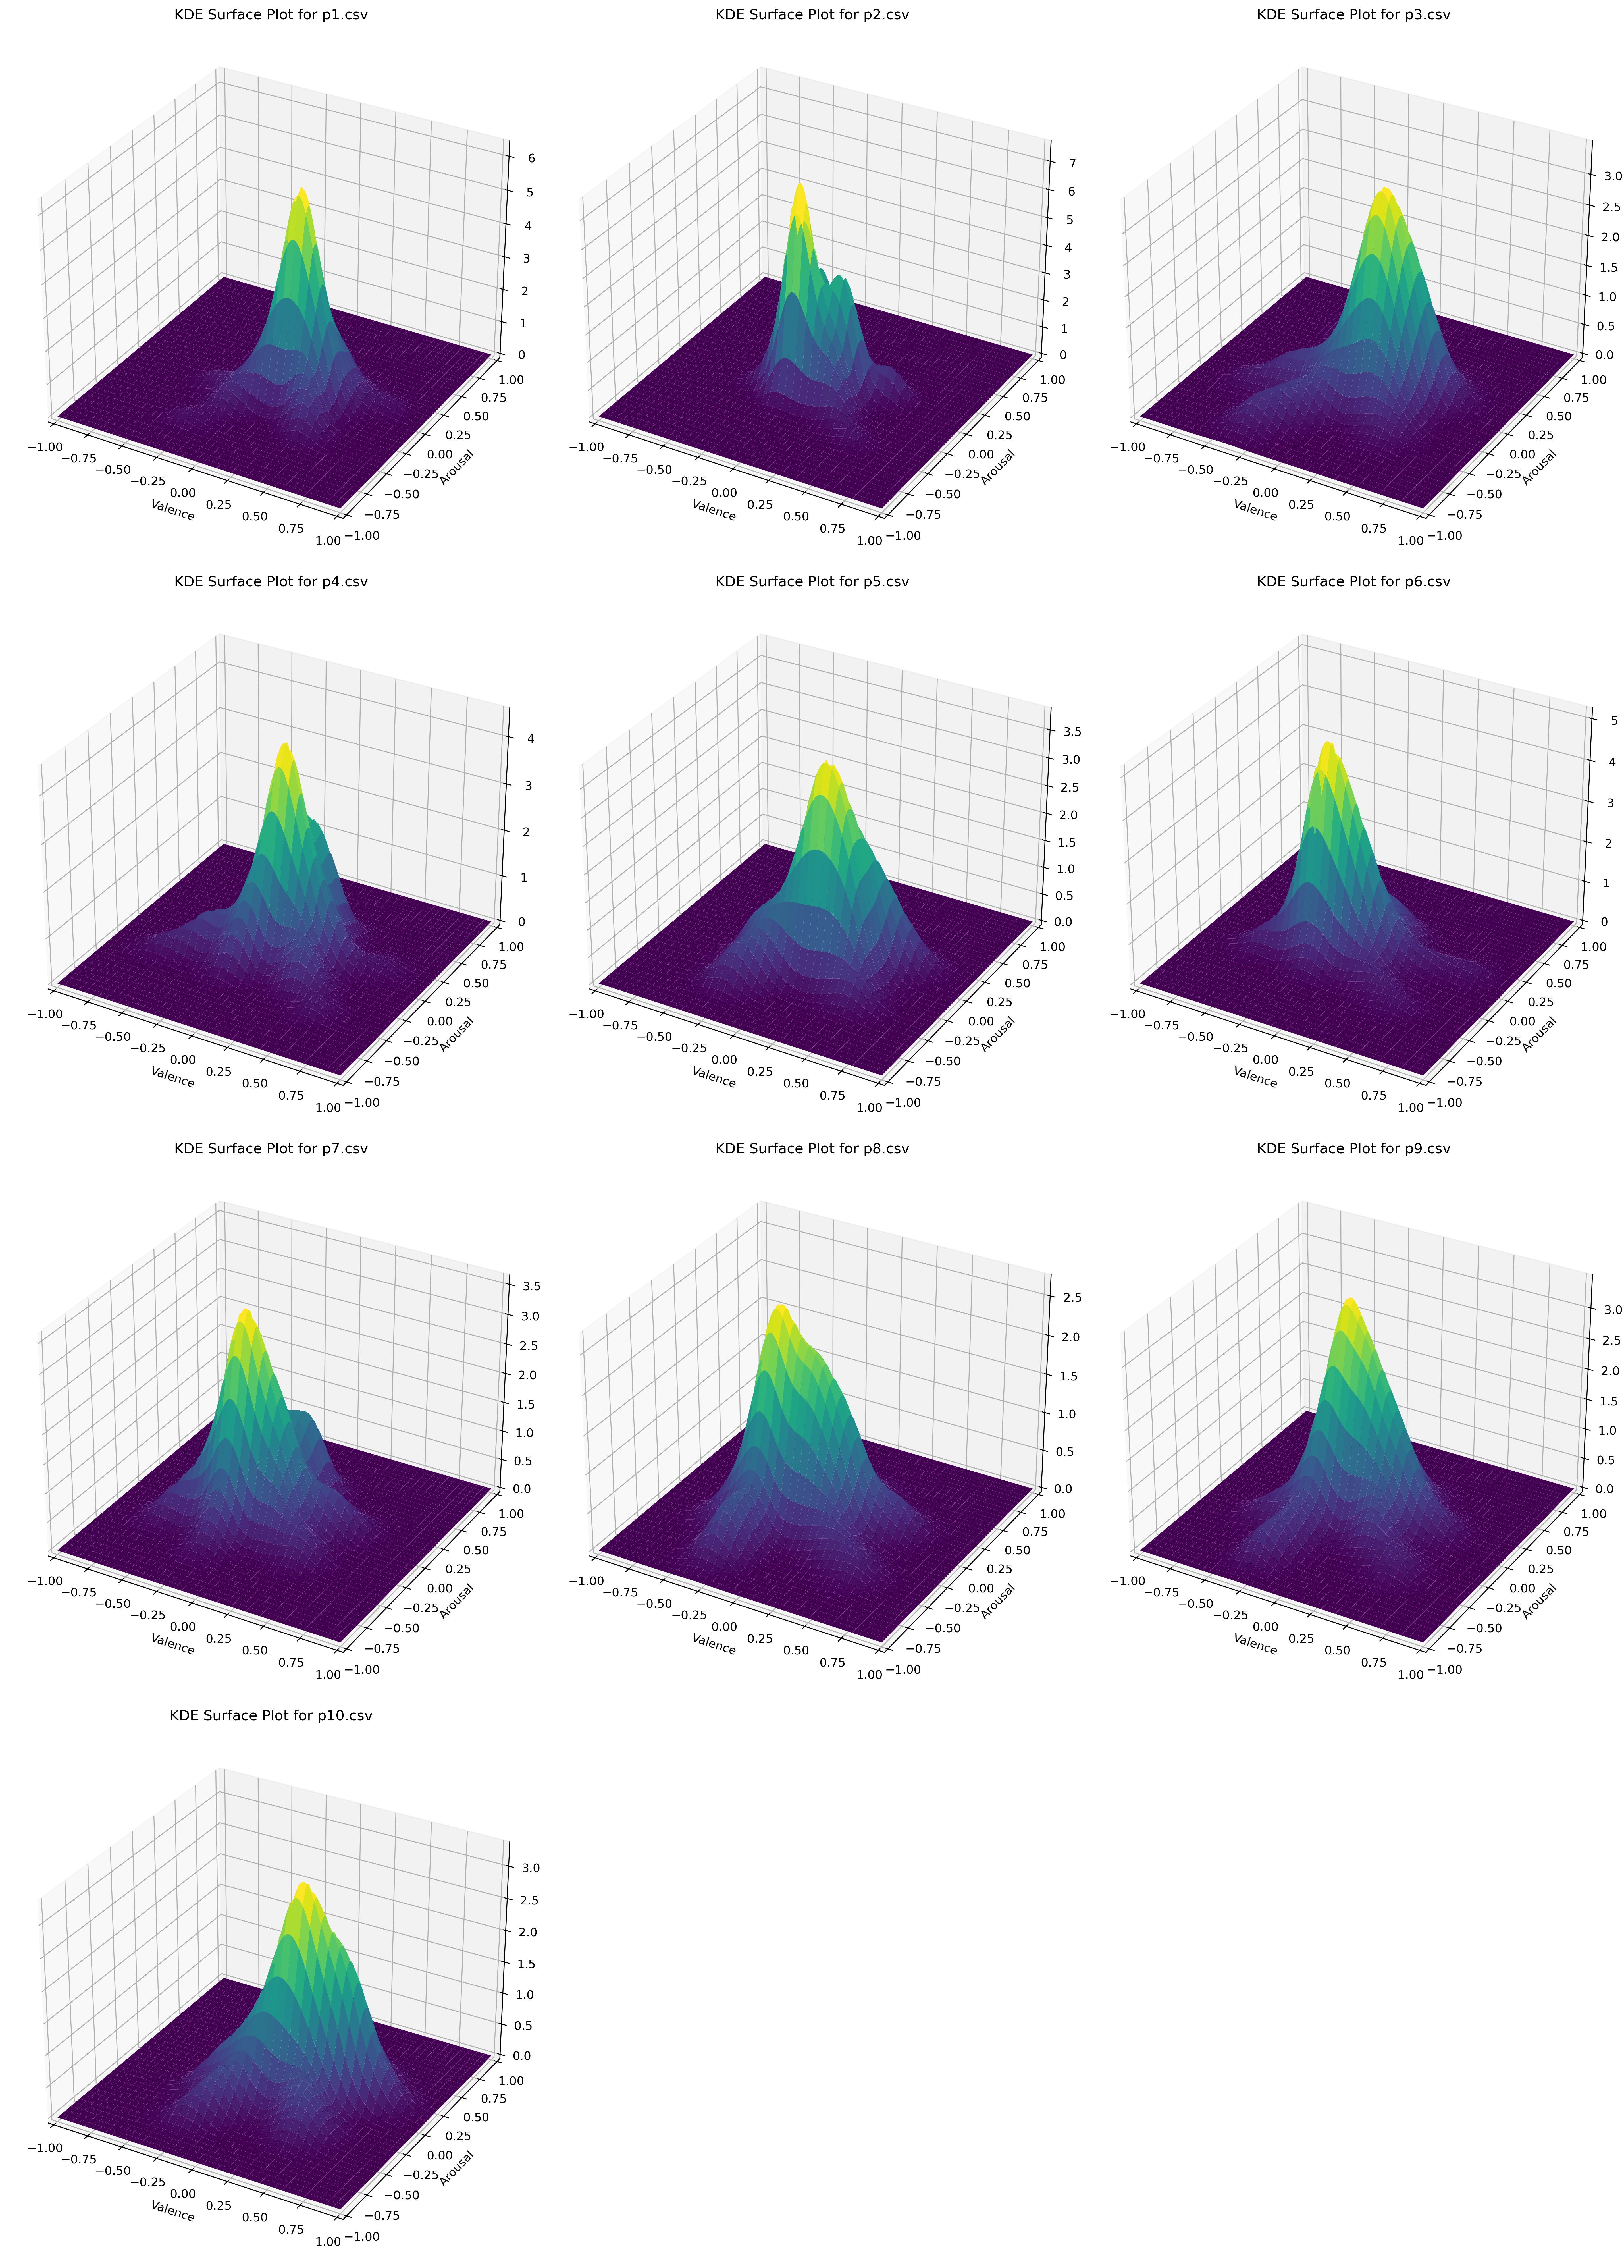
\includegraphics[width=0.80\textwidth]{img/chapter_04/baseline/kde_surface_all-new.png}
    \caption{3D surface plots of KDE-based emotional distributions for all participants}
    \label{fig:kde-3d-plots}
\end{figure}


\begin{figure}[H]
    \centering
    \includegraphics[width=0.80\textwidth]{img/chapter_04/baseline/kde_2d_baseline_map-new.png}
    \caption{2D mapping of KDE-estimated baseline zones for each participant}
    \label{fig:kde-2d-baselines}
\end{figure}


\subsection*{Evaluation}

To evaluate the accuracy and relevance of the identified baseline values, we conducted a questionnaire with all participants. Each participant was asked to reflect on the emotional states represented in their baseline region and indicate how closely those states matched their typical emotional condition during the experiment sessions.

The full questionnaire and participant responses are provided in the Appendix (see Section~\ref{sec:appendix-questionnaire}). Based on the collected responses, we calculated the frequency of agreement between the participants and the computed baseline zones. This frequency distribution is shown in Figure~\ref{fig:baseline-agreement-bar}, which highlights the overall agreement levels across all participants.

In addition, we visualized the relationship between the identified baselines and the participants’ self-reported emotional states using a valence-arousal scatter plot. This comparison, presented in Figure~\ref{fig:baseline-scatter-plot}, helps illustrate how closely the KDE-based baseline aligns with the participants' own perception.

\begin{figure}[H]
    \centering
    \includegraphics[width=0.75\textwidth]{img/chapter_04/baseline/agreement_bar.png}
    \caption{Participant agreement frequency with identified baseline values}
    \label{fig:baseline-agreement-bar}
\end{figure}

\begin{figure}[h]
    \centering
    \includegraphics[width=1\textwidth]{img/chapter_04/baseline/valence_arousal_scatter.png}
    \caption{Scatter plot comparing identified and participant-proposed baseline coordinates}
    \label{fig:baseline-scatter-plot}
\end{figure}


The analysis of the questionnaire responses provides valuable insights into the accuracy and acceptance of the computed baseline values. 

\textbf{General Agreement Level:} The mean agreement score for Question 1  was 3.70 out of 5, indicating that most participants tended to agree with their computed emotional baseline. Furthermore, 60\% of participants explicitly expressed agreement, which supports the reliability of the baseline computation method for the majority.

\textbf{Baseline Discrepancy:} To measure how much the participants’ proposed baselines differed from the computed values, we used the Euclidean distance.
The mean distance was found to be 0.120 with a standard deviation of 0.122. This result shows that, on average, participants' self-identified baseline points differ from the computed values by around 0.12 units in the valence-arousal space. The similarity between the mean and standard deviation also indicates a consistent pattern in how much the computed and proposed baselines deviate from each other. Table~\ref{tab:agreement_summary} summarizes the computed distances for each participant.

\begin{table}[H]
    \centering
    \caption{Participant Agreement and Baseline Discrepancy Summary}
    \begin{tabular}{lcccc}
    \toprule
    \textbf{Participant ID} & \textbf{Agreement (1-5)} & \textbf{Proposed (Valence, Arousal)} & \textbf{Distance} \\
    \midrule
    P1 & 4 & (0.25, -0.05) & 0.054 \\
    P2 & 3 & (0.40, -0.02) & 0.230 \\
    P3 & 4 & (0.20, 0.10) & 0.305 \\
    P4 & 5 & (0.23, -0.06) & 0.014 \\
    P5 & 3 & (-0.05, 0.15) & 0.071 \\
    P6 & 4 & (0.35, -0.10) & 0.054 \\
    P7 & 2 & (0.20, 0.20) & 0.321 \\
    P8 & 4 & (0.24, -0.07) & 0.014 \\
    P9 & 3 & (0.10, -0.05) & 0.134 \\
    P10 & 5 & (0.21, -0.10) & 0.000 \\
    \bottomrule
    \end{tabular}
    \label{tab:agreement_summary}
    \end{table}
    
\section{Phase 4: LLM Response Evaluation}
\label{sec:phase4-llm-evaluation}

In this phase, participants were asked to evaluate the responses generated by the language model based on the procedure outlined in Section~\ref{sec:phase4-llm-responses}. The responses were assessed using a Likert scale across four criteria: \textit{Relevance}, \textit{Emotional Alignment}, \textit{Empathy}, and \textit{Satisfaction}. Each participant rated responses to both a standard (controlled) query and an emotionally-enhanced query.

This evaluation allowed us to compare how the emotional enhancement influenced user perception of the generated responses. The comparison of average ratings between the two types of queries across all four evaluation dimensions is illustrated in Figure~\ref{fig:llm_eval_comparison}.

\begin{figure}[h]
    \centering
    \includegraphics[width=1\textwidth]{img/chapter_04/llm/mean_ratings_comparison.png}
    \caption{Comparison of average ratings for LLM responses}
    \label{fig:llm_eval_comparison}
\end{figure}

\subsection*{Overall Analysis Results}

\begin{table}[H]
    \centering
    \begin{tabular}{|l|c|c|c|c|}
    \hline
    \textbf{Dimension} & \textbf{\makecell{Mean\\Control}} & \textbf{\makecell{Mean\\Enhanced}} & \textbf{\makecell{Mean\\Difference}} & \textbf{\makecell{Improvement\\(\%)}} \\
    \hline
    Satisfaction        & 3.343 & 4.600 & 1.257 & 37.6 \\
    Empathy             & 2.200 & 3.857 & 1.657 & 75.3 \\
    Emotional Alignment & 2.343 & 3.971 & 1.629 & 69.5 \\
    Relevance           & 3.743 & 3.814 & 0.071 & 1.9  \\
    \hline
    \end{tabular}
    \caption{Comparison of participant evaluations for control vs emotionally enhanced responses}
    \label{tab:llm_overall_analysis}
\end{table}


As seen in Table~\ref{tab:llm_overall_analysis}, there is a clear overall increase in user satisfaction, indicating a robust and consistent enhancement in user experience when emotional tailoring is applied. This suggests that emotionally enhanced responses are more engaging and fulfilling for users across various types of queries.

The most significant improvements are observed in \textit{Empathy} (75.3\%) and \textit{Emotional Alignment} (69.5\%), followed by \textit{Satisfaction} (37.6\%). These dimensions, being closely linked to subjective and emotional user experiences, benefit substantially from emotional enhancement. 

On the other hand, the impact on \textit{Relevance} is limited. With only a 1.9\% improvement and a low proportion of participants reporting a positive change as relevance is more dependent on content correctness, which was already adequately addressed by the control responses.

\section{Phase 5: Baseline Refinement}
\label{sec:baseline-refinement}

Following the initial baseline identification, we selected a subset of participants whose self-identified baselines aligned closely with the computed values. This selection was based on their agreement level. The selected participants included P1, P4, P6, P8, and P10. We conducted initial training using those datapoints available around baseline region. 

Subsequently, data was collected during the refinement tasks described in Paragraph~\ref{par:refineing-tasks}.Then observed about the baseline shofts. Initial and refine baseline regions are illustrated in Figure~\ref{fig:baseline-refine-all} for above participants.

\begin{figure}[h]
    \centering
    \includegraphics[width=1\textwidth]{img/chapter_04/b-refine/baseline-refine-all.png}
    \caption{Initial and refined baseline regions for selected participants.}
    \label{fig:baseline-refine-all}
\end{figure}


The results of this section are detailed in Appendix \ref{sec:appendix-refine-questionnaire}, where participant feedback on the refined baselines was collected. As shown in the table, the agreement scores and refined baseline coordinates were evaluated using a Likert scale. Out of the six participants, four (P1, P3, P4, and P6) rated the refined baselines with a score of 4 or higher, indicating agreement with the computed values. This reflects a 66.67\% agreement rate, suggesting that the refined baseline identification method was successful for the majority of users.

\begin{table}[H]
\centering
\caption{Participant Agreement on Refined Baselines}
\begin{tabular}{|c|p{5cm}|c|}
\hline
\textbf{PID} & \textbf{Refined Baseline (V, A)} & \textbf{Likert Score} \\
\hline
P1 & [(0.3, -0.1), (0.4, -0.2)] & 4 \\
P3 & [(0.2, -0.1), (0.3, -0.2)] & 5 \\
P4 & [(0.1, 0.1), (0.2, 0.0)] & 5 \\
P6 & [(-0.2, 0.0), (-0.1, -0.1)] & 4 \\
P8 & [(0.1, 0.2), (0.2, 0.1)] & 2 \\
P10 & [(0.3, -0.1), (0.4, -0.2)] & 3 \\
\hline
\end{tabular}
\end{table}



% CONCLUSION
\section{Conclusion}
This chapter summarizes the key findings of the research by revisiting the research aim and questions, highlighting the contributions made, and discussing limitations and possible future directions. Section~\ref{sec:conclusion-rq} provides a summary of how each research question was addressed through the different stages of the study. Section~\ref{sec:research-contributions} outlines the main contributions of this work, including the personalized multimodal fusion approach and the novel baseline identification mechanism. Finally, Section~\ref{sec:limitations-future-work} discusses the limitations of the current study and suggests several directions for future research to improve and expand the system further.

\section{Conclusions about the Research Questions and Aim}
\label{sec:conclusion-rq}

\par The main aim of this research was to develop a personalized emotion recognition system using facial and vocal signals, and to integrate these emotional insights into LLM responses to make them more emotionally intelligent. The research was divided into five stages, and each stage focused on addressing specific research questions and objectives.

\par In the first stage, several pre-implemented facial and vocal emotion recognition models were compared to answer \hyperref[rq:1.1]{RQ 1.1} (What are suitable pre-implemented models that can be used to get a higher accuracy for emotion recognition?). Between HUME and CAGE for facial expression, HUME scored considerably higher overall. In the case of audio models, both HUME Audio and Wave2Vec2 showed different strengths, but the performance gap between them was smaller compared to facial models. We selected the HUME model for both modalities to maintain consistency. This model selection helped to lay a strong foundation for building a multimodal framework.

\par In the second stage, we addressed \hyperref[rq:1.2]{RQ 1.2} (How the recognized emotion values from different modalities fused together in order to get more personalized arousal-valence value?) by fusing the facial and vocal predictions using decision-level fusion. Mean Squared Error was used to calculate the weights for fusion. The fused predictions showed lower average Euclidean distance compared to using either facial or vocal data alone, especially in cases where one modality was weaker. This means the fused model was more accurate and closely matched the ground truth emotions.

\par The third stage focused on identifying an initial emotional baseline to answer \hyperref[rq:2.1]{RQ 2.1} (What techniques are most suitable for establishing an initial emotional baseline and how can this baseline be dynamically adjusted over time to reflect changes in the user's emotional responses and self-reported feedback?). We used Kernel Density Estimation based on participant data. To verify accuracy, we collected feedback from participants through a questionnaire. The average agreement score was 3.70 out of 5, showing that most users agreed with the identified baseline values.
 
\par In the fourth stage, we evaluated how emotional input could change the output of a LLM model. We used GPT-4o-mini and found a noticeable increase in user satisfaction when emotional context was included with user queries. This confirms the value of emotionally aware responses and successfully answers \hyperref[rq:3.1]{RQ 3.1} (How does integrating personalized emotional state information with user queries affect the relevance and user satisfaction of responses from LLMs?).

\par Finally, in the fifth stage, we revisited the emotional baseline and used reinforcement learning to refine it over time. Among six participants, four rated the refined baseline with 4 or higher out of 5, giving a 66.67\% agreement rate. This result shows that the method works for most users and improves personalization over time, again supporting \hyperref[rq:2.1]{RQ 2.1}.

\par Overall, this research shows that using personalized emotional state recognition with facial and audio data can meaningfully improve how LLMs respond to users. The findings give a starting point for building emotionally aware AI systems and highlight areas for future improvements like larger datasets, longer-term user adaptation, and better real-time emotion tracking.

\section{Research Contributions}
\label{sec:research-contributions}

\par This research provides several key contributions in the area of personalized emotion recognition and emotionally aware AI systems. The focus was on building a system that works differently for each user by understanding their unique emotional patterns through both facial and vocal signals.

\begin{itemize}
    \item \paragraph*{Personalized Emotion Recognition using MSE-based Fusion} One of the main contributions is the implementation of a personalized multimodal emotion recognition method. This was done by combining facial and vocal predictions using a decision-level fusion approach. The weights were calculated based on the MSE between the predicted values and user self-reported emotions. This personalized approach was applied for identifying five target emotions: Happy, Angry, Sad, Boredom, and Calm.

    \item \paragraph*{Emotional Baseline Identification in Arousal-Valence Plane} Another key contribution is the method used to identify each user's emotional baseline in the arousal-valence space. KDE was used on the collected data to estimate a stable starting point for each participant’s emotional state.

    \item \paragraph*{Baseline Refinement using Emoji-Based Feedback Mechanism} A novel method was introduced to refine the baseline over time using user feedback. Instead of traditional methods, participants gave feedback using simple emoji-based inputs. These responses were used in a reinforcement learning loop to adjust the emotional baseline.

\end{itemize}

\par These contributions together help to create a more personalized and emotionally intelligent interaction between users and AI systems. They also offer a foundation for future work in real-time and long-term emotion tracking systems for individuals.

\section{Limitations and Future Work}
\label{sec:limitations-future-work}

This research focused on five basic emotions (Happy, Angry, Sad, Boredom, and Calm) which helped build the core of the system, but these do not fully represent the entire arousal-valence plane. Including a wider range of emotional categories like fear, surprise, or mixed emotions would make the system more complete and useful in real-life applications. Also, the use of only facial and vocal signals may not capture the full complexity of human emotions. Previous studies suggest that physiological signals such as EEG, ECG, and GSR can provide deeper emotional insights and should be explored in future versions. The fusion process in this research was based on a statistical MSE approach, which showed promising results, but more advanced fusion methods like deep learning-based techniques could offer better personalization and flexibility depending on the situation. In terms of emotional baseline estimation, machine learning models can be used to enhance the current KDE-based approach and allow the system to learn and adapt more effectively over time. Lastly, since the experiments were conducted with a small group of participants from similar backgrounds, future work should focus on involving more diverse users in terms of age, language, and culture to ensure the system performs well across different populations.

% ACKNOWLEDGMENTS
\section*{Acknowledgments}
The authors would like to thank the University of Moratuwa for their support.

% CRediT AUTHOR STATEMENT
\section*{CRediT author statement}
Avishka Sathyanjana: Conceptualization, Methodology, Formal analysis, Writing – original draft preparation.

% REFERENCES
\newpage
\bibliography{refernce/references}

\end{document}